%%%%%%%%%%%%%%%%%%%%%%%%%%%%%%%%%%%%%
%% Projeto Final - Arquivo principal
%% UNIVERSIDADE C�NDIDO MENDES - Bacharel em Ci�ncias da Computa��o
%% Projeto final: M�dulo de Mapeamento do Toolkit H�rus.
%% J�natas Oliveria Lopes Soares / Maycon Barreto Lopes / Wallace Gomes de Souza
%% Orientador: Prof. D. �talo Matias
%% Campos dos Goytacazes - RJ
%% 2009
%%%%%%%%%%%%%%%%%%%%%%%%%%%%%%%%%%%%%%

\documentclass[a4paper,12pt]{report}

\usepackage{a4wide}
\usepackage[brazil,english]{babel}
\usepackage[dvips]{graphicx}
\usepackage{amsmath}
\usepackage{epsfig}
\usepackage[latin1]{inputenc}
\usepackage{doublespace}
\usepackage{fancyheadings}
\usepackage{longtable}
\usepackage{dropping}
\usepackage{url}
\usepackage{subfigure}
\usepackage{abntcite}
\def\citeopen{[}
\def\citeclose{]}

\newcommand{\figr}[1]{Figura~\ref{#1}}
\newcommand{\eqt}[1]{Eq.~(\ref{#1})}
\newcommand{\eqts}[2]{Eq.~(\ref{#1})~e~(\ref{#2})}
\newcommand{\eqtss}[3]{Eq.~(\ref{#1})~,~(\ref{#2})~e~(\ref{#3})}
\newcommand{\tab}[1]{Tabela~\ref{#1}}

%comandos para se definir cabe�alhos nas p�ginas da disserta��o
\pagestyle{fancyplain}
\lhead[\fancyplain{}{\thepage}]{\fancyplain{}{\small\leftmark}}
\rhead[\fancyplain{}{\small\rightmark}]{\fancyplain{}{\thepage}}
\cfoot{\fancyplain{\thepage}{}}

%package para uso de verbatimtab

%configura��o para numera��o de subsubse��es
\setcounter{secnumdepth}{3}

\newcounter{mypage}

% Frases de efeito no in�cio de cada cap�tulo
\newcommand{\epigraph}[2]{%
  \vspace{1ex}%
  {\footnotesize%
   \begin{spacing}{1}
    \begin{flushright}%
      \begin{minipage}{.6\textwidth}%
        #1\\
      \end{minipage}\\
      \textit{#2}%
    \end{flushright}
    \end{spacing}}%
  \vspace{1ex}}

\DeclareGraphicsExtensions{.jpg, .pdf, .mps, .png}

\begin{document}
 \stepcounter{mypage}

%--------------------------------
%  PRIMEIRAS P�GINAS
%--------------------------------
%%%%%%%%%%%%%%%%%%%%%%%%%%%%%%%%%%%%%
%% Projeto Final - Arquivo principal
%% UNIVERSIDADE C�NDIDO MENDES - Bacharel em Ci�ncias da Computa��o
%% Projeto final: M�dulo de Mapeamento do Toolkit H�rus.
%% J�natas Oliveria Lopes Soares / Maycon Barreto Lopes / Wallace Gomes de Souza
%% Orientador: Prof. D. �talo Matias
%% Campos dos Goytacazes - RJ
%% 2009
%%%%%%%%%%%%%%%%%%%%%%%%%%%%%%%%%%%%%%


\thispagestyle{empty}

\begin{spacing}{1.0}

\begin{center}
\begin{large}
UNIVERSIDADE C�NDIDO MENDES
\end{large}
\end{center}

\vspace {2 cm}
\begin{center}
\begin{large}
\uppercase{
J�natas Oliveria Lopes Soares \par Maycon Barreto Lopes \par Wallace Gomes de Souza
}
\end{large}
\end{center}
\vspace {4 cm}
\begin{spacing}{1.5}
\begin{center}
\begin{huge}
{\bf \uppercase{
M�dulo de Mapeamento do ToolKit H�rus}
}
\end{huge}

\end{center}
\end{spacing}

\vspace {8 cm}

\begin{center}

\begin{large}
Campos dos Goytacazes - RJ \\[0.2 cm]
2009
\end{large}
\end{center}

\end{spacing}
\newpage




\stepcounter{mypage}
%%%%%%%%%%%%%%%%%%%%%%%%%%%%%%%%%%%%%
%%   Folha de rosto
%%%%%%%%%%%%%%%%%%%%%%%%%%%%%%%%%%%%%


\thispagestyle{empty}

\begin{spacing}{1.0}

\begin{center}
\begin{large}
\uppercase{
Chrystiano Barbosa de Souza Ara�jo \par Leandro Moraes Vale Cruz \par Lucas Carvalho Teixeira \par Thiago Ribeiro Nunes} \\[0.2 cm]
\end{large}
\end{center}

\vspace {5 cm}

\begin{spacing}{1.5}
\begin{center}
\begin{Large}
{\bf \uppercase{Aspectos de Vis�o Computacional no desenvolvimento do \textit{toolkit} Horus}}
\end{Large}
\end{center}
\end{spacing}

\vspace {2 cm}

\begin{flushright}
\begin{minipage}[t]{8.5 cm}
Monografia apresentada � Universidade C�ndido Mendes como requisito obrigat�rio para a obten��o do grau de Bacharel em Ci�ncias da Computa��o.
\end{minipage}
\end{flushright}

\vspace {1.5 cm}

\begin{center}
\begin{large}
ORIENTADOR: Prof. D.Sc. �talo de Oliveira Matias\\[0.2 cm]
\end{large}
\end{center}

\begin{center}
\begin{large}
CO-ORIENTADOR: Prof. D.Sc. Dalessandro Soares Vianna\\[0.2 cm]
\end{large}
\end{center}

\vspace {1.5 cm}

\begin{center}
\begin{large}
Campos dos Goytacazes-RJ\\[0.2 cm]
2009
\end{large}
\end{center}

\end{spacing}
\newpage


\stepcounter{mypage}
%%%%%%%%%%%%%%%%%%%%%%%%%%%%%%%%%%%%%
%%   Folha de aprova��o
%%%%%%%%%%%%%%%%%%%%%%%%%%%%%%%%%%%%%


\thispagestyle{empty}

\begin{spacing}{1.0}

\begin{center}
\end{center}

\vspace {1.0 cm}

\begin{center}
\begin{Large}
{\bf \uppercase{Aspectos de Vis�o Computacional no desenvolvimento do \textit{toolkit} Horus}
} \\[0.2 cm]
\end{Large}
\end{center}

\vspace {1.0 cm}

\begin{flushright}
\begin{minipage}[t]{8.5 cm}
Monografia apresentada � Universidade C�ndido Mendes como requisito obrigat�rio para a obten��o do grau de Bacharel em Ci�ncias da Computa��o.
\end{minipage}
\end{flushright}

\vspace {1.5 cm}

\begin{center}
\begin{large}
Aprovada em \_\_\_\_ de \_\_\_\_\_\_\_\_\_\_\_\_ de 2009. \\[0.2 cm]
\end{large}
\end{center}

\vspace {1.5 cm}

\begin{center}
\begin{large}
BANCA EXAMINADORA \\[0.2 cm]
\end{large}
\end{center}

\vspace {1 cm}

\begin{center}
\line(1,0){300}\\ 
Prof. �talo de Oliveira Matias - Orientador \\
D.Sc.em Sistemas Computacionais pela UFRJ\\

\end{center}

\vspace {1.0 cm}

\begin{center}
\line(1,0){300}\\ 
Prof. Dalessandro Soares Vianna\\
D.Sc. em Inform�tica pela PUC-Rio
\end{center}

\vspace {1.0 cm}

\begin{center}
\line(1,0){300}\\ 
Prof. Ferm�n Alfredo Tang Montan�\\
D.Sc. em Engenharia de Produ��o pela UFRJ
\end{center}

\end{spacing}
\newpage

\stepcounter{mypage}
%%%%%%%%%%%%%%%%%%%%%%%%%%%%%%%%%%%%%
%%  DEDICAT�RIA
%%%%%%%%%%%%%%%%%%%%%%%%%%%%%%%%%%%%%


\thispagestyle{empty}

\

\vfill

\begin{flushright}
\hfill \textit{Dedico este trabalho a minha m�e \\
 J�natas}
\vspace*{1cm}

\textit{
Dedico este trabalho a meus pais
\\ Maycon}

\vspace*{1cm}

\textit{
Dedico este trabalho a meus pais
\\ Wallace}

\end{flushright}

\vspace*{1cm}

\clearpage

\stepcounter{mypage}
%%%%%%%%%%%%%%%%%%%%%%%%%%%%%%%%%%%%%
%%  AGRADECIMENTOS
%%%%%%%%%%%%%%%%%%%%%%%%%%%%%%%%%%%%%


\chapter*{Agradecimentos}
\thispagestyle{empty}
Agradecemos as nossas fam�lias e amigos, pela paci�ncia e apoio, que possibilitou calma e for�as para o desenvolvimento desse projeto, assim como durante todos os momentos dif�ceis ao longo de nossa gradua��o. Agradecemos aos orientadores Italo de Oliveira Matias e Dalessandro Soares Vianna pelo apoio e orienta��o para o desenvolvimento desse trabalho, assim como a Universidade Candido Mendes por propiciar um ambiente frut�fero a pesquisa e aprendizado.


\thispagestyle{empty} 


% Caso passe de p�gina adicionar essa linha para  que n�o seja reformatada
% inserir o restante do texto abaixo dela.
% \thispagestyle{empty} 


\stepcounter{mypage}
%\include{epigrafe}


%-----------------------------------
% DOCUMENTA��O DO TRABALHO
%-----------------------------------

\renewcommand{\baselinestretch}{1.3}
%-----------------------------------
% NUMERA��O DE P�GINA EM ROMANO
%-----------------------------------

\pagenumbering{roman}
\setlength{\voffset}{0.0in}

% Atribui ao contador page (default do latex, que � usado por todo o documento)
% o valor do nosso contador mypage
\setcounter{page}{\value{mypage}}

\begin{spacing}{1.5}
%%%%%%%%%%%%%%%%%%%%%%%%%%%%%%%%%%%%%
%%   Resumo
%%%%%%%%%%%%%%%%%%%%%%%%%%%%%%%%%%%%%


\chapter*{Resumo}



\vspace{0.5cm}

Palavras-chave: 

\end{spacing}

\begin{spacing}{1.5}
%%%%%%%%%%%%%%%%%%%%%%%%%%%%%%%%%%%%%
%%   Abstract
%%%%%%%%%%%%%%%%%%%%%%%%%%%%%%%%%%%%%


\chapter*{Abstract}
This work presents the concepts and algorithms involved in the construction of an Open Source toolkit, named Horus, used in development and control of applications involving intelligent agents, focusing on two central problems. The first problem relates to the handling of autonomous intelligent agent in unknown environments. The second problem relates to computer vision, where the agent should be able to extract information from the environment through the use of virtual or real cameras. In addition to algorithms for computer vision and autonomous movement, the Horus also provides abstractions for the development and configuration of intelligent agents with their main components and devices. While Horus was also developed with a focus on movement of autonomous intelligent agents, this work is focused on the computer vision algorithms and abstractions for creation and configuration of intelligent agents. As a proof of concept and validation of the functionality provided by the toolkit Horus, were also developed three distinct applications: PyANPR, Teseu and Ariadnes. PyANPR is an automatic number plate recognition web system. Teseu is a system that simulates the automatic mapping of an unknown environment by an intelligent agent. Ariadnes is a system that simulates the movement of an autonomous intelligent agent in an unfamiliar environment using techniques of computer vision and unknown environments mapping. This work will also detail the PyANPR application and the computer vision aspects of the Ariadnes simulator.


\vspace{0.5cm}

Keywords: Computer Vision, Environment Mapping, Horus


\end{spacing}

\selectlanguage{brazil}

\begin{spacing}{1.0}
\tableofcontents
\listoffigures
\listoftables
\end{spacing}

\clearpage

% Atribuindo ao nosso contador o valor do contador page
% e depois incremento...
\setcounter{mypage}{\value{page}}
\clearpage

\pagenumbering{arabic}

\begin{spacing}{1.5}
\setcounter{page}{\value{mypage}} % Atribuindo o contador page novamente....
%%%%%%%%%%%%%%%%%%%%%%%%%%%%%%%%%%%%%
%%   Introdu��o
%%%%%%%%%%%%%%%%%%%%%%%%%%%%%%%%%%%%%


\chapter{Introdu��o}

Existem alguns tipos de ambiente que s�o in�spitos ao homem. Nesses casos � comum utilizar rob�s para explorar e atuar em tais locais. A movimenta��o desses rob�s pode ser autom�tica (agentes aut�nomos), semi-autom�tica (agentes semi-aut�nomos) ou manual. Neste trabalho, ser�o apresentados os passos para a constru��o de um \textit{toolkit Open Source} , de nome Horus, utilizado para o desenvolvimento e controle de aplica��es que envolvam agentes inteligentes, com foco em dois problemas centrais. O primeiro problema refere-se � movimenta��o aut�noma de um agente inteligente em ambientes desconhecidos. O segundo problema refere-se �  vis�o computacional, onde o agente deve ser capaz de extrair informa��es do ambiente atrav�s da utiliza��o de c�meras virtuais ou reais.

Um Agente, por defini��o, � todo elemento ou entidade aut�noma que pode perceber seu ambiente, por algum meio cognitivo ou sensorial, e de agir sobre esse ambiente por interm�dio de atuadores. Podem-se citar como exemplos de agentes inteligentes, al�m de rob�s aut�nomos ou semi-aut�nomos, personagens de um jogo, agentes de busca e recupera��o de informa��o, entre outros.

Para que um agente aut�nomo seja capaz de atuar em um ambiente desconhecido � necess�rio anteriormente explorar esse local. Essa explora��o pode ser feita atrav�s de um mapeamento desse ambiente. A forma como se mapeia o ambiente internamente no sistema � determinante na sua precis�o e performance. As diferentes abordagens para controle de agentes m�veis aut�nomos interagem fortemente com a representa��o do ambiente. Uma proposta para o mapeamento do ambiente, ainda n�o implementada no Horus, consiste na constru��o de um ambiente virtual 3D associado a um ambiente real no qual um rob� real est� explorando. Essa abordagem exige que o agente reconhe�a padr�es no ambiente explorado e represente-os no ambiente virtual. 

 Durante a explora��o do ambiente nos simuladores constru�dos, o agente dever� ser capaz de estimar sua posi��o local para localizar-se globalmente e se recuperar de poss�veis erros de localiza��o. Um correto mapeamento do ambiente junto a aplica��o correta das leis da cinem�tica pode resolver tal problema. Uma proposta para a localiza��o de um agente no ambiente � a utiliza��o do m�todo Monte Carlo \cite{FOX1999} ou do m�todo SLAM (\textit{Simultaneous Location and Mapping}) \cite{Davison2004}, \cite{Dellaert2005}. O m�todo selecionado para ser implementado no \textit{toolkit} Horus foi o SLAM.

 Um agente explora um ambiente atrav�s de sensores. O sensoriamento prov� ao rob� as informa��es necess�rias para a constru��o de uma representa��o do ambiente onde est� inserido e para uma intera��o com os elementos contidos nesse. Sistemas com uma variedade de sensores tendem a obter resultados mais precisos. A fus�o de dados de sensores, ou como � mais conhecida, fus�o de sensores, � o processo de combina��o de dados de m�ltiplos sensores para estimar ou predizer estados dos elementos da cena. Neste trabalho, foram utilizados lasers, c�meras e od�metro como sensores.

 Para simular a vis�o de um agente inteligente, s�o utilizadas c�meras virtuais. Na abordagem desse trabalho, a vis�o � a principal forma de percep��o do ambiente. A vis�o possibilita reconhecer padr�es e classificar obst�culos.
Existem diferentes tipos de obst�culos. Estes podem ser classificados como transpon�vel (aquele que n�o interrompe a trajet�ria), intranspon�vel (aquele que o exigir� recalcular a trajet�ria por outro caminho) e redutor (aquele que permite o rob� seguir pela trajet�ria, por�m a uma velocidade mais lenta). Mesmo mediante a obst�culos transpon�veis e redutores, pode ser conveniente recalcular o caminho devido ao aumento do custo do percurso. Uma proposta para o desvio de trajet�ria � o modelo baseado em Campos Potenciais proposto por [8]. A classifica��o de um obst�culo ocorre mediante a algum m�todo de reconhecimento de padr�es, baseado em vis�o computacional.

O \textit{toolkit} Horus, criado neste trabalho, prop�e uma cole��o de classes e algoritmos voltados a resolu��o de problemas pertencentes as �reas de vis�o computacional e mapeamento autom�tico de ambientes. Nessa monografia, ser� dado foco � parte de vis�o computacional do Horus. De forma a validar a implementa��o desse \textit{toolkit} e demonstrar a sua utilidade, foram desenvolvidas tr�s aplica��es distintas: Os simuladores Teseu e Ariadnes, e o PyANPR. Neste trabalho, al�m do \textit{toolkit} Horus, ser�o, tamb�m, apresentados a parte de vis�o computacional utilizada no simulador Ariadnes e a aplica��o para reconhecimento autom�tico de placas de autom�veis PyANPR.


%%%%%%%%%%%%%%%%%%%%%%%%%%%%%%%%%%%%%
%%  Extra��o de Caracter�sticas
%%%%%%%%%%%%%%%%%%%%%%%%%%%%%%%%%%%%%


\chapter{Intelig�ncia Computacional}
\label{cap:ia}

\section{Agentes Inteligentes}
A Intelig�ncia Computacional (IC) � uma �rea de estudo da ci�ncia da computa��o que procura desenvolver sistemas computacionais capazes de ter a��es e rea��es similares as capacidades humanas, tais como: pensar, criar, solucionar problemas entre outros. Um Agente, por defini��o, � todo elemento ou entidade aut�noma que pode perceber seu ambiente por algum meio cognitivo ou sensorial e de agir sobre esse ambiente por interm�dio de atuadores \cite{Russel2003}. Pode-se citar como exemplos de agentes inteligentes, al�m de um rob� aut�nomo ou semi-aut�nomo, personagens de um jogo, agentes de busca e recupera��o de informa��o e agentes de chats.

Existem diferentes defini��es para a arquitetura de um rob� presentes na literatura. Este trabalho considera a defini��o abordada por Arkin cite(Ark98) a qual considera que uma arquitetura de um rob� est� mais relacionada com os aspectos de software que os de hardware. Apesar de algumas diferen�as, os modelos de arquitetura para rob�s m�veis descrevem um mecanismo para constru��o de um sistema de desenvolvimento e controle de agentes inteligentes, apresentando, principalmente, quais os m�dulos presentes e como estes interagem. 

De uma forma geral, os m�dulos de uma arquitetura de um agente inteligente se preocupam com aspectos como percep��o, planejamento e atua��o$/$execu��o. A percep��o refere-se � compreens�o do ambiente e dos elementos nele contido. Denomina-se \textit{sequ�ncia de percep��es}, a hist�ria completa de tudo que o agente j� percebeu, ou seja, o conjunto de todas as percep��es do agente at� um dado momento; o planejamento � intelig�ncia do rob�; e a atua��o, ou execu��o, � o modo como o rob� procede no ambiente, ou seja, movimentos, captura de informa��es, etc.

Existem diversos modelos de arquitetura para rob�tica entre os quais ressalta-se os modelos de tr�s camadas como: SSS cite(CON92), Atlantis cite(Gat91), 3T cite{Bon91}. Todas as arquiteturas se dividem semelhantemente da seguinte forma:

    
\begin{itemize}
	\item camada reativa: orienta os sensores e atuadores, al�m de tomar decis�es de baixo n�vel, como vis�o e movimento;
	\item camada deliberativa: respons�vel pela intelig�ncia do rob�, aspectos mais globais, que n�o s�o alterados a cada itera��o;
	\item camada de execu��o: intermedia essas duas outras camadas.
\end{itemize}
 
As camadas reativa e deliberativa prov�em processos denominados de comportamentos. Em termos matem�ticos, o comportamento do agente � a fun��o que mapeia qualquer percep��o ou sequ�ncia de percep��es para uma a��o espec�fica \cite{Russel2003}, essa fun��o � conhecida como \textit{fun��o de agente}. 

Com base nesses conceitos, definiu-se neste trabalho um agente como uma entidade composta de comportamentos, dispositivos e um programa de agente. Os dispositivos do agente, utilizados no sistema em quest�o, s�o de sensoriamento (lasers e c�meras) e de movimenta��o (rodas). Os comportamentos do agente s�o: mapeamento, navega��o e reconhecimento de objetos. O programa de agente � respons�vel pelo controle da execu��o de todos os comportamentos supracitados.

 Os comportamentos s�o procedimentos implementados para representar a��es e rea��es dos agentes. As a��es s�o comportamentos ativos, ou seja, procedimentos que visam realizar um objetivo previamente definido. Por outro lado, rea��es s�o procedimentos realizados mediante a est�mulos externos. Exemplos de a��o e rea��o ocorrem no deslocamento de um agente de uma posi��o a outra. Para realizar o deslocamento � necess�rio tra�ar uma rota. Tal comportamento � definido como uma a��o. Ao se deparar com algum obst�culo durante o percurso, esse agente deve gerar um comportamento de replanejamento da rota para alcan�ar o objetivo inical sem colidir com o obst�culo. A esse replanejamento, denomina-se rea��o.

	Comportamentos podem ser divididos em duas categorias. Os Comportamentos Prim�rios: parar, reduzir velocidade, acelerar, desviar de obst�culos, virar, inverter dire��o, dirigir-se a meta, fotografar, disparar lasers e etc; e Comportamentos Inteligentes: mapear, reconhecer objetos, navegar e executar uma tarefa espec�fica. Um Comportamento Inteligente executa um conjunto de comportamentos Prim�rios para atingir seu objetivo. Os comportamentos prim�rios ocorrem na camada reativa, enquanto que, os inteligentes ocorrem na camada deliberativa.

Entende-se por \textit{Programa de Agente} o programa que recebe as percep��es do ambiente como entrada e as mapeia para uma determinada a��o atrav�s da fun��o de agente. Al�m da estrutura citada, o programa de agente pode ser estruturado de outras maneiras. Um exemplo de estrutura � construir o programa de agente como um conjunto de sub-rotinas que ser�o executadas de forma ass�ncrona em rela��o ao ambiente. O programa permanece em \textit{loop}, recebendo todas as percep��es geradas pelo ambiente, e repassa cada percep��o para uma sub-rotina que ir� trat�-la.

Os programas de agente podem ser classificados em quatro categorias principais:
\begin{itemize}
	\item Agentes reativos simples: esse tipo de programa de agente se basea apenas na percep��o atual para executar as suas a��es, onde a sequ�ncia de percep��es at� o momento � ignorada.
	
	\item Agentes reativos baseados em modelo: esse programa de agente armazena uma sequ�ncia de percep��es e toma suas decis�es levando em considera��o as percep��es dessa sequ�ncia.
	
	\item Agentes baseados em objetivos: esse programa de agente possui informa��es sobre o objetivo que deve alcan�ar. Logo, suas decis�es s�o tomadas com base na combina��o das percep��es do ambiente e nas informa��es do objetivo.

	\item Agentes baseados na utilidade: esse tipo de programa de agente tem a preocupa��o, n�o s� de alcan�ar o seu objetivo final, como tamb�m em determinar a melhor forma poss�vel de alcan��-lo. 
\end{itemize}

Em duas das aplica��es desenvolvidas neste trabalho, os programas de agente utilizados se enquadram na categoria de agentes baseados na utilidade.

\section{Reconhecimento de Padr�es}
\label{sec:recObj}
Reconhecimento de padr�es � um atividade que os humanos fazem a todo tempo e, normalmente, sem um esfor�o consciente. Seres humanos recebem informa��es atrav�s de v�rios sensores org�nicos, as quais s�o processadas instantaneamente pelo c�rebro. Essa habilidade � ainda mais impressionante no que diz respeito a assertividade do processo de reconhecimento mesmo quando as informa��es n�o se encontram em condi��es ideais, como por exemplo, em situa��es onde as informa��es s�o vagas, imprecisas, ou at� mesmo, incompletas.
	A �rea de Reconhecimento de Padr�es � respons�vel por projetar algoritmos e abordagens  que procuram aproximar as tarefas realizadas computacionalmente das habilidades humanas. Esse processo consiste em classificar e descrever objetos atrav�s de um conjunto de caracter�sticas ou propriedades. Um dos principais conceitos dentro de reconhecimento de padr�es � o discriminante.  Tal conceito consiste em medir uma dist�ncia de um determinado padr�o para cada outro previamente conhecido. Logo, a classe de um determinado padr�o ser� a mesma do seu vizinho mais pr�ximo [Simp 92], [Simp 93], de menor dist�ncia ou o prot�tipo mais parecido [Torb 98].
    	Espera-se de um  sistema de reconhecimento de padr�es que este seja capaz de aprender de uma forma adaptativa e din�mica. Em sistemas de reconhecimento de padr�es autom�ticos, as etapas de aprendizagem e reconhecimento s�o combinados a fim de atingir um objetivo desejado [Cagn 93] [Valli 98]. Portanto, redes neurais artificiais � uma das principais t�cnicas utilizadas nesse sentido [Nigr 93] e ser� apresentada na se��o \ref{sec:rna}.
 	Um t�pico sistema de reconhecimento de padr�o consiste em tr�s partes: aquisi��o de dados, sele��o$/$extra��o de caracter�sticas e classifica��o$/$clustering [Pattern recognition book].

\begin{itemize}
\item Aquisi��o de dados: � o processo de sele��o dos dados que ser�o usados como entrada no processo de reconhecimento. Tais dados podem ser qualitativos, quantitativos ou ambos. Podendo ser num�ricos, lingu�sticos, entre outros. 

\item Sele��o$/$Extra��o de caracter�sticas: o objetivo principal desta etapa consiste em gerar o melhor conjunto de caracter�sticas necess�rias para o processo de reconhecimento, de modo a maximizar a efic�cia do sistema.  A grande dificuldade dessa etapa est� na determina��o de um crit�rio adequado para a escolha de um bom conjunto de caracter�sticas. Um bom crit�rio � aquele que � imut�vel para qualquer varia��o poss�vel dentro de uma classe, todavia, deve ser capaz de destacar as diferen�as importantes a fim de discriminar entre diferentes tipos de padr�es.

\item Classifica��o$/$clustering: classifica��o � o processo de defini��o de qual classe um determinado padr�o de entrada pertence. Essa classifica��o pode ser feita utilizando t�cnicas determin�sticas e probabil�sticas. As classes s�o definidas a partir de um conjunto de amostras apresentadas na etapa de aprendizagem.

\end{itemize}

A t�cnica de reconhecimento de padr�es possui uma grande variedade de aplica��es. Dentre elas, pode-se citar: reconhecimento de faces, leitura biom�trica, identifica��o de circuitos impressos defeituosos, reconhecimento �ptico de caracteres, reconhecimento de fala e de escrita cursiva, entre outros.


\section{Redes Neurais Artificiais}
\label{sec:rna}
Redes Neurais Artificiais (RNAs) s�o estruturas computacionais que visam imitar a forma com que o c�rebro humano processa as informa��es. O c�rebro possui a capacidade de organizar e encadear seus elementos estruturais, conhecidos como neur�nios, para realizar o processamento das informa��es de forma n�o linear e paralela. Dessa forma, as principais caracter�sticas das redes neurais s�o a habilidade de aprender rela��es complexas e n�o lineares entre os padr�es de entrada e as sa�das, utilizarem procedimentos de treinamento seq�encial e se auto-adaptar aos dados \cite{Jain2000}.

	Na sua forma geral, uma rede neural � uma m�quina projetada para imitar a forma com que o c�rebro realiza uma tarefa particular ou uma fun��o de interesse, podendo ser implementada em hardware ou simulada atrav�s de software. Para atingir uma performance razo�vel, as redes neurais empregam uma massiva interconex�o de unidades de processamento simples, denominadas neur�nios \cite{Haykin1994}. 

As redes neurais artificais possuem a capacidade de aprendizado e, como conseq��ncia, de generaliza��o. Generaliza��o refere-se � produ��o de sa�das racionais para entradas que n�o foram apresentadas a rede durante a fase de treinamento ou aprendizado. As capacidades de aprendizado e de generaliza��o tornam as redes neurais capazes de resolver problemas complexos e n�o-lineares. A seguir, ser�o explicadas algumas caracter�sticas do neur�nio biol�gico, fundamentais para o entendimento das RNAs.

\subsection{Neur�nio Biol�gico}

O sistema nervoso � formado por um conjunto extremamente complexo de neur�nios. Os neur�nios est�o conectados uns aos outros atrav�s de sinapses. Nos neur�nios a comunica��o � realizada atrav�s de impulsos el�tricos, quando um impulso � recebido, o neur�nio o processa, e passado um limite de a��o, dispara um segundo impulso o qual flui do corpo celular para o ax�nio que, por sua vez, pode ou n�o estar conectado a um dendrito de outra c�lula. A Figura \ref{fig:neuroBiol} apresenta uma representa��o de um neur�nio.

\begin{figure}[!htb]
\centering
\begin{center}
    \includegraphics[scale=0.35, bb= 0 0 751 469]{imagens/neuronioBio.PNG}
\end{center}
\caption{Neur�nio biol�gico}
\label{fig:neuroBiol}
\end{figure}

Os principais componentes de um neur�nio s�o:
\begin{itemize}
\item Os dendritos: membrana que recebe os est�mulos gerados por outras c�lulas. Os dendritos s�o as entradas do neur�nio.

\item Soma: � o corpo do neur�nio, que � respons�vel por coletar e combinar informa��es vindas de outros neur�nios;

\item O ax�nio: membrana constitu�da de uma fibra tubular que � respons�vel por transmitir os est�mulos para outras c�lulas. O ax�nio representa a sa�da do neur�nio.
\end{itemize}

O neur�nio biol�gico � constitu�do de um corpo celular denominado soma. Nesse Local ocorre o processamento metab�lico da c�lula nervosa ou neur�nio. A partir da soma, projetam-se extens�es filamentares denominadas dendritos, e o ax�nio. Este modelo anat�mico foi identificado por Ramon Cajal em 1894. Com base nas pesquisas de Erlanger e Gasser, em 1920, e outras posteriores, passou-se a entender o comportamento do neur�nio biol�gico como sendo o dispositivo computacional do sistema nervoso, o qual possui muitas entradas e uma �nica sa�da \cite{Haykin1994}.

	As entradas ocorrem atrav�s das conex�es sin�pticas, que conectam a �rvore dendrital aos ax�nios de outras c�lulas nervosas. Os sinais que chegam pelos dendritos s�o pulsos el�tricos conhecidos como impulsos nervosos ou potenciais de a��o, e constituem a informa��o que o neur�nio processar� de alguma forma para produzir como sa�da um impulso nervoso no seu ax�nio.

	Sinapse � o nome dado ao ponto de contato entre a termina��o ax�nica de um neur�nio e o dendrito de outro.  � pelas sinapses que os nodos se unem funcionalmente, formando a rede neural.  As sinapses funcionam como v�lvulas, e s�o capazes de controlar a transmiss�o de impulsos entre os nodos na rede \cite{Braga2000} e est�o compreendidas entre duas membranas celulares: a membrana pr�-sin�ptica, que recebe o est�mulo vindo de uma c�lula, e a membrana p�s-sin�ptica, que � a do dendrito. Na regi�o pr�-sin�ptica, se o est�mulo nervoso recebido atinge um determinado limiar em um espa�o curto de tempo, a c�lula "dispara", produzindo um impulso que � transferido para outras c�lulas atrav�s de neurotransmissores presentes na membrana dendrital. Dependendo do neurotransmissor, a conex�o sin�ptica � excitat�ria ou inibit�ria. A conex�o excitat�ria provoca uma altera��o no potencial da membrana que contribui para forma��o do impulso nervoso no ax�nio de sa�da, enquanto que a conex�o inibit�ria age no sentido contr�rio.

	O mecanismo como � criado o potencial de a��o ou impulso nervoso � o seguinte: quando o potencial da membrana est� menos eletronegativo do que o potencial de repouso, diz-se que a membrana est� despolarizada e quando est� mais negativo, diz-se que ela est� hiperpolarizada. O impulso nervoso ou potencial de a��o � uma onda de despolariza��o de certa dura��o de tempo, que se propaga ao longo da membrana. A forma��o de um potencial de a��o na membrana axonal ocorre quando essa membrana sofre despolariza��o suficientemente acentuada para cruzar um determinado valor conhecido como limiar de disparo. Quando esse limiar � superado, os est�mulos s�o passados para outras c�lulas atrav�s das liga��es sin�pticas.

\subsection{O Neur�nio Artificial MCP}
McCulloch e Pits \cite{Mendel1970} propuseram um modelo matem�tico do neur�nio artificial MCP. Esse modelo foi proposto com base nos principais conceitos do neur�nio biol�gico. O modelo matem�tico do neur�nio proposto por McCulloch e Pits apresenta n terminais de entrada $x_1, x_2, ..., x_n$ (representando os dendritos) e apenas um terminal de sa�da $y$ (representando o ax�nio). Os terminais de entrada do neur�nio t�m pesos acoplados $w_1,w_2, ..., w_n$ cujos valores podem ser positivos ou negativos caso as sinapses correspondentes serem inibit�rias ou excitat�rias. O efeito de uma sinapse particular $i$ no neur�nio p�s-sin�ptico � dado por $x_i w_i$. Os pesos determinam o n�vel em que o neur�nio deve considerar sinais de disparo que ocorrem naquela conex�o. Uma descri��o do modelo est� ilustrada na Figura \ref{fig:mcculloch}.

\begin{figure}[!htb]
\centering
\begin{center}
    \includegraphics[scale=0.4, bb= 0 0 349 264]{imagens/mcculloch.PNG}
\end{center}
\caption{Modelo do neur�nio de McCulloch e Pits}
\label{fig:mcculloch}
\end{figure}

O corpo do neur�nio realiza um simples somat�rio dos valores $x_iw_i$ que chegam a ele. Se o somat�rio dos valores ultrapassa o limiar de ativa��o ou \textit{threshold}, o neur�nio dispara (valor 1 na sa�da), caso contr�rio o neur�nio permanece inativo (valor 0 na sa�da). A ativa��o do neur�nio � realizada atrav�s de uma fun��o de ativa��o, que dispara ou n�o o neur�nio dependendo do valor da soma ponderada das suas entradas. No modelo MCP original, a fun��o de ativa��o ativar� a sa�da quando:

\begin{center}


$\sum_{i=1}^{n} x_{i}w_{i} \geq \theta$


\end{center}

Na equa��o acima, $n$ � a quantidade de entradas do neur�nio, $w_i$ � o peso associado � entrada $x_i$ e $\theta$ � o limiar do neur�nio.

\subsection{Fun��es de Ativa��o}
A partir do modelo apresentado por McCulloch e Pits, surgiram v�rios outros modelos que permitem a produ��o de qualquer sa�da, n�o apenas zero ou um, e com v�rias fun��es de ativa��o. As fun��es de ativa��o mais comuns s�o: 


\begin{itemize}
\item Fun��o Limiar: fun��o utilizada no modelo de McCulloch e Pits, caracterizada por "tudo ou nada", representada da seguinte forma:   \[ f(v) = \left\{
                                 \begin{array}{ll}
                                     1,  $ v $ \geq 0\\
                                     0,  $ v $ \leq 0
                                 \end{array}
                           \right. \]



Onde $v$ � igual ao valor produzido pelo somat�rio das entradas do neur�nio. 

\begin{figure}[!htb]
\centering
\begin{center}
  \includegraphics[scale=0.35, bb= 0 0 300 222]{imagens/graficoFuncaoLimiar.PNG}
\end{center}
\caption{Gr�fico da fun��o Limiar}
\label{fig:fLimiar}
\end{figure}


\item Fun��o Sigm�ide: essa � uma fun��o semilinear, limitada e monot�nica que pode assumir valores entre $0$ e $1$. Existem v�rias fun��es sigmodais, por�m, a mais usada � a fun��o log�stica definida pela equa��o: 

\begin{center}
    $f(v) = \frac{1}{1+e^{(-av)}}$
\end{center}

Onde $a$ � o par�metro de inclina��o da fun��o sigm�ide e $v$ � o valor de ativa��o do neur�nio.

\begin{figure}[!htb]
\centering
\begin{center}
 \includegraphics[scale=0.35, bb= 0 0 290 220]{imagens/graficoFuncaoSigmoide.PNG}
\end{center}
\caption{Gr�fico da fun��o sigm�ide}
\label{fig:funcSignum}
\end{figure}

\item Fun��o Signum: essa fun��o apresenta as mesmas caracter�sticas da fun��o limiar, por�m, se limita ao intervalo entre $1$ e $-1$. Essa fun��o � representada por:  

\begin{center}
    $f(v) = b\frac{v}{|v|} $ para $ v \neq 0$
\end{center}

Onde $b$ s�o os limites inferiores e superiores $(b = |1|$ no gr�fico$)$ e $v$ � o valor de ativa��o.

\begin{figure}[!htb]
\centering
\begin{center}
 \includegraphics[scale=0.35, bb= 0 0 280 208]{imagens/graficoFuncaoSignun.PNG}
\end{center}
\caption{Gr�fico da fun��o Signum}
\label{fig:graficoSignum}
\end{figure}

\item Tangente Hiperb�lica: seu gr�fico � parecido com o da Fun��o Sigm�ide, assumindo valores entre $1$ e $-1$, sendo representada por:

\begin{center}
    $f(v) = a\frac{e^{(bv)} - e^{(-bv)}}{e^{(bv)} + e^{(bv)}} $
\end{center}

Onde a � o par�metro de inclina��o da curva, b s�o os limites inferiores e superiores $(b = |1|$ no gr�fico$)$ e $v$ o valor de ativa��o.

\begin{figure}[!htb]
\centering
\begin{center}
\includegraphics[scale=0.35, bb= 0 0 279 207]{imagens/graficoHiperbolica.PNG}
\end{center}
\caption{Gr�fico da Tangente Hiperb�lica}
\label{fig:graficoHiperbolica}
\end{figure}

\end{itemize}



\subsection{Arquiteturas de Redes Neurais}
A defini��o da arquitetura de uma RNA define a maneira com que os neur�nios s�o estruturados na rede \cite{Haykin1994}. A arquitetura restringe o tipo de problema que pode ser tratado pela rede. Redes com uma camada �nica de nodos MCP, por exemplo, s� conseguem resolver problemas linearmente separ�veis. Redes recorrentes, por sua vez, s�o mais apropriadas para resolver problemas que envolvem processamento temporal \cite{Braga2000}. A arquitetura de uma rede � definida pelos seguintes par�metros: n�mero de camadas da rede, n�mero de neur�nios em cada camada, tipo de conex�o entre os neur�nios e topologia da rede.
	
Em geral, as redes neurais podem ser classificadas quanto ao n�mero de camadas, quanto ao tipo de conex�o e quanto � conectividade entre os neur�nios. Quanto ao n�mero de camadas t�m-se:

\begin{itemize}
\item Redes de uma �nica camada: existe apenas um n� entre uma entrada e uma sa�da da rede. A Figura \ref{fig:unicacamada} apresenta um exemplo de redes de �nica camada.

\begin{figure}[htb]
\centering
\begin{center}
    \includegraphics[scale=0.45, bb= 0 0 125 123]{imagens/redeUmaCamada.PNG}
\end{center}
\caption{Redes de uma �nica camada}
\label{fig:unicacamada}
\end{figure}

\item Redes de m�ltiplas camadas: existe mais de um neur�nio entre alguma entrada e alguma sa�da (Figura \ref{fig:multiplaCamada}).

\begin{figure}[!htb]
\centering
\begin{center}
    \includegraphics[scale=0.45, bb= 0 0 171 103]{imagens/redeMultiplaCamada.PNG}
\end{center}
\caption{Rede de m�ltiplas camadas}
\label{fig:multiplaCamada}
\end{figure}
\end{itemize}

Quanto ao tipo de conex�o t�m-se:

\begin{itemize}
\item Feedforward, ou ac�clica: a sa�da de um neur�nio na $i$-�sima camada da rede n�o pode ser usada como entrada de nodos em camadas de �ndice menos ou igual a $i$ Figura \ref{fig:unicacamada}.

\item Feedback, ou c�clica: a sa�da de algum neur�nio na $i$-�sima camada da rede � utilizada como entrada em neur�nios da camada de �ndice menor ou igual a $i$ (Figura \ref{fig:feedback}).

\begin{figure}[!htb]
\centering
\begin{center}
    \includegraphics[scale=0.45, bb= 0 0 182 115]{imagens/feedBack.PNG}
\end{center}
\caption{Exemplo de rede feedback.}
\label{fig:feedback}
\end{figure}

Quanto � conectividade t�m-se:

\begin{itemize}
\item Redes parcialmente conectadas (Figura \ref{fig:unicacamada}).
\item Redes completamente conectadas (Figura \ref{fig:multiplaCamada}).

\end{itemize}

\subsection{Processo de aprendizado}
	A principal propriedade de uma rede neural � a sua habilidade de aprender sobre o ambiente no qual est� inserida de forma a melhorar a sua performance na resolu��o de problemas complexos. Essa melhora na performance � adquirida a cada instante do processo de aprendizado de acordo com uma forma de medi��o pr�-estabelecida. Com isso, uma rede neural aprende sobre seu ambiente atrav�s de um processo iterativo de ajuste dos pesos sin�pticos adquirindo mais conhecimento sobre o problema ap�s cada itera��o do processo de aprendizado.
	Segundo Mendel e McLaren \cite{Mendel1970}, no contexto de redes neurais, aprendizado � o processo pelo qual os par�metros de uma rede neural s�o ajustados atrav�s de est�mulos produzidos pelo ambiente no qual a rede est� inserida. O tipo de aprendizado � determinado pela maneira particular com que os par�metros s�o modificados.
	Foram desenvolvidos diversos m�todos de treinamento de redes, podendo ser agrupados em dois paradigmas principais: aprendizado supervisionado e aprendizado n�o-supervisionado. No entanto, outros dois paradigmas bastante conhecidos s�o os de aprendizado por refor�o (que � um caso particular de aprendizado supervisionado) e aprendizado por competi��o (que � um caso particular de aprendizado n�o supervisionado). 

\begin{itemize}
\item Aprendizado Supervisionado:


Esse tipo de aprendizado � o mais utilizado em RNAs. Esse aprendizado � dito supervisionado porque as entradas e as respectivas sa�das desejadas s�o fornecidas por um supervisor externo, normalmente chamado de "professor". Seu objetivo � ajustar os pesos da rede, de forma a encontrar uma liga��o entre os pares de entrada e sa�da fornecidos pelo professor.
	O professor � respons�vel por direcionar o processo de aprendizado fornecendo os padr�es de entrada, as sa�das desejadas e a taxa de erro desejada.  A cada padr�o de entrada submetido � rede pelo professor, compara-se a resposta desejada (que representa uma solu��o �tima para aquele padr�o de entrada) com a resposta calculada, ajustando-se os pesos das conex�es para minimizar o erro. A minimiza��o da diferen�a � incremental, j� que pequenos ajustes s�o feitos nos pesos a cada itera��o do aprendizado. A soma dos erros quadr�ticos de todas as sa�das � normalmente utilizada como medida de desempenho da rede e tamb�m como fun��o de custo a ser minimizada pelo algoritmo de treinamento. A Figura \ref{fig:aprendSuper} apresenta um esquema b�sico de aprendizado supervisionado.

\begin{figure}[!htb]
\centering
\begin{center}
    \includegraphics[scale=0.45, bb= 0 0 348 211]{imagens/aprendizadoSupervRNA.PNG}
\end{center}
\caption{Esquema de aprendizado supervisionado.}
\label{fig:aprendSuper}
\end{figure}

Nesse trabalho, o algoritmo de aprendizado utilizado foi o \textit{backpropagation}.


\item Aprendizado N�o Supervisionado:


No aprendizado n�o supervisionado n�o h� um professor que oriente o processo de aprendizado. Ao contr�rio do aprendizado supervisionado, que possui pares de entrada e sa�da, para esses algoritmos somente s�o disponibilizados os padr�es de entrada. De acordo com as regularidades estat�sticas com que as entradas ocorrem, a rede cria classes de acordo com as caracter�sticas extra�das de cada padr�o de entrada. Dessa forma, para cada entrada fornecida a rede, a sa�da ser� a classe a qual a entrada pertence.  Caso a entrada n�o perten�a a nenhuma classe pr�-existente, a rede cria uma nova classe para essa entrada. A base para a utiliza��o desse tipo de aprendizado � a redund�ncia nos dados, sem redund�ncia, seria praticamente imposs�vel a utiliza��o bem sucedida do aprendizado n�o supervisionado. A Figura \ref{fig:aprendNaoSuper} apresenta um esquema de um sistema de aprendizado n�o supervisionado.

\begin{figure}[!htb]
\centering
\begin{center}
    \includegraphics[scale=0.4, bb= 0 0 445 93]{imagens/aprendizadoNSuper.PNG}
\end{center}
\caption{Esquema de aprendizado n�o supervisionado.}
\label{fig:aprendNaoSuper}
\end{figure}


\end{itemize}
\section{Computa��o Gr�fica}

	A computa��o gr�fica � a ci�ncia que basicamente estuda um conjunto de t�cnicas que transforma dados em imagem apresentada atrav�s de um dispositivo gr�fico. Estes dados podem ser organizados atrav�s de um modelo matem�tico cuja geometria se assemelhe a do objeto do mundo real a qual se deseja modelar. Segundo J. Gomes e L.Velho em \cite{Gomes2003} a computa��o gr�fica pode ser dividida em quatro sub-�reas que relacionam dados e imagens. Essas sub�reas s�o t�o pr�xima que est�o muitas vezes interligadas, em determinados momentos s�o at� confundidas. Estas sub-�reas s�o: Modelagem Geom�trica, S�ntese de Imagem, Processamento de Imagem e Vis�o Computacional. A figura \ref{fig:CG} mostra estas quatro sub-�reas da computa��o gr�fica e como se relacionam com os dados e a imagem: 

\begin{figure}[!htb]
\centering
\begin{center}
    \includegraphics[scale=0.4, bb= 0 0 564 398]{imagens/CG.PNG}
\end{center}
\caption{Sub-�reas da computa��o gr�fica}
\label{fig:CG}
\end{figure}

	A Modelagem Geom�trica trata do problema de descrever e estruturar dados geom�tricos no computador, ou seja, encontrar um modelo matem�tico capaz de representar o objeto desejado. Um exemplo de Modelagem geom�trica � a obten��o de uma fun��o que se aproxime de outra desconhecida atrav�s de um m�todo de interpola��o de alguns pontos de amostragem j� conhecidos.
	
	A S�ntese de imagens, ou Visualiza��o, processa os dados gerados pelo sistema na modelagem geom�trica e produz uma imagem que pode ser vista em um dispositivo de sa�da gr�fica. A partir do mapeamento de alguns pontos, distribu�dos em torno de um determinado objeto, obt�m-se um modelo matem�tico, que o representa, atrav�s da Modelagem Geom�trica. De posse deste modelo � poss�vel apresentar uma imagem que represente a forma do objeto. Este �ltimo processo � um exemplo de S�ntese de Imagem.
	
	O Processamento de Imagens assume como dados de entrada uma imagem, processa-a produzindo uma outra imagem como dado de sa�da. As t�cnicas desta �rea podem ser utilizadas, por exemplo, para melhorar a qualidade de uma imagem antiga ou danificada, produzindo outra, imagem com menos ru�dos.
	
	Por �ltimo, o processo de Vis�o Computacional, ou simplesmente Vis�o, tem por finalidade obter, a partir de uma imagem de entrada, informa��es f�sicas, geom�tricas e/ou topol�gicas sobre os dados do objeto apresentado na imagem. Um bom exemplo desta �rea aparece nas transmiss�es de futebol, quando � necess�rio observar com seguran�a e certeza se um jogador est� em posi��o de impedimento, ou seja, uma situa��o onde � necess�rio determinar a sua posi��o no campo em rela��o � posi��o dos jogadores advers�rios.
	
	Para determinados pesquisadores a Computa��o Gr�fica � apenas a �rea denominada de s�ntese de imagem. Por�m para \cite{Gomes2003}, al�m de outros pesquisadores desta �rea, esta ci�ncia � composta pelas quatro linhas apresentadas acima. Este fato se justifica gra�as ao fato de cada vez surgir mais m�todos e t�cnicas que solucionem problemas nestas quatro vertentes.
	

\section{Vis�o Computacional}
Vis�o computacional � uma linha de pesquisa que procura definir procedimentos automatizados que imitem processos da vis�o humana (ou de outros animais).  Normalmente essa �rea basea-se em t�cnicas estat�sticas, ou probabil�sticas, para estimar informa��es baseadas em imagens. Para desenvolver t�cnicas nessa linha de pesquisa � essencial uma boa compreens�o sobre o funcionamento das c�meras (com suas falhas na aquisis�o de sinais que comp�em uma imagem, inser��o de ru�dos, distor��o de cores, etc) assim como seu posicionamento no espa�o ambiente. Esse segundo problema � conhecido como calibra��o de camera e � um tema largamente estudado, pois normalmente, para estimar informa��es em uma cena vista em duas dimens��es � necess�rio ter no��es sobre profundidade (e profundidade � estimada atrav�s da especifica��o da posi��o da c�mera e de objetos na cena).

De um modo mais geral vis�o computacional � a �rea da computa��o gr�fica que extrai informa��es de uma imagem ou de um conjunto de imagens. Existem diversas aplica��es de vis�o computacional em diversas �reas como detec��o autom�tica de tumores imagens m�dicas; defini��o de posi��o de jogadores de futebol no campo, em um determinado instante; determina��o de volume de um fluido em mares ou rios, etc.

Nesse trabalho foi estudado um tema particular de vis�o computacional, que � o de reconhecimento de padr�es, se��o \ref{sec:recObj}. Para reconhecer padr�es, assim como na maioria dos problemas de vis�o computacional, � necess�rio extrair caracter�sticas da imagem.

Um padr�o em particular que podemos citar s�o caracteres. O campo de pesquisa, dentro da vis�o computacional, que se preocupa com o reconhecimento de caracteres � conhecido pelo acr�nimo OCR, do ingl�s, Optical Recognition Caracter. Esse tema ser� abordado na se��o \ref{sec:ocr}.

\subsection{Extra��o de caracter�sticas}

No campo de reconhecimento de padr�es, extrair caracer�sticas significa extrair medidas associadas ao objeto que se deseja reconhecer, de forma que essas medidas sejam semelhantes para objetos semelhantes e diferentes para objetos distintos \cite{Santos2007}. Definir vetores de caracter�sticas � o m�todo para representa��o de dados mais comum e conveniente para problemas de classifica��o e reconhecimento. Cada caracter�stica resulta de uma medi��o qualitativa ou quantitativa, que � uma vari�vel ou um atributo do objeto [Guyon et al., 2006] .
    Para reconhecer um caractere de uma representa��o bitmap, h� a necessidade de extrair caracter�sticas do mesmo para descrev�-lo de uma forma mais apropriada para o seu processamento computacional e reconhecimento. Como o m�todo de extra��o de caracter�sticas afeta significantemente a qualidade de todo o processo de reconhecimento de padr�es, � muito importante extrair caracter�sticas de modo que elas sejam invariantes no que diz respeito �s v�rias condi��es de ilumina��o, tipo de fonte e poss�veis deforma��es dos caracteres causadas, por exemplo, pela inclina��o da imagem. 
    
       Geralmente, a descri��o de uma regi�o de uma imagem � baseada em suas representa��es interna e externa. A representa��o interna de uma imagem � baseada em suas propriedades regionais, como cor ou textura. A representa��o externa � selecionada quando se deseja dar �nfase nas caracter�sticas da forma do objeto. Logo, o vetor de caracter�sticas de uma representa��o externa inclui caracter�sticas como o n�mero de linhas, a quantidade de arestas horizontais, verticais e diagonais, etc.
        
        O conjunto de vetores de caracter�sticas forma um espa�o vetorial. Cada caractere representa uma determinada classe, e todas as formas de representa��o desse caractere definem as inst�ncias dessa classe. Todas as inst�ncias do mesmo caractere devem ter uma descri��o similar atrav�s de vetores num�ricos chamados de "descritores", ou "padr�es". Logo, vetores suficientemente pr�ximos representam o mesmo caractere. Essa � a premissa b�sica para que o processo de reconhecimento de padr�es seja bem sucedido.

No cap�tulo que trata do \textit{toolkit} Horus, ser�o explicados alguns m�todos de extra��o de caracter�sticas implementados no m�dulo de vis�o computacional.

\subsection{Reconhecimento �ptico de Caracteres}
\label{sec:ocr}

Reconhecimento �ptico de Caracteres ou OCR (\textit{Optical character recoginition}) � um campo de pesquisa nas �reas de reconhecimento de padr�es, intelig�ncia artificial e vis�o computacional. Em computa��o, OCR � o processo de tradu��o eletr�nica de imagens de textos para textos que possam ser editados computacionalmente, permitindo assim, a realiza��o de opera��es que seriam invi�veis de serem realizadas sobre o texto em formato de imagem. Sistemas OCR, ou de reconhecimento de caracteres, datam do final dos anos 50 e t�m sido amplamente utilizados em computadores desktop desde os anos 90.
	Esses sistemas disponibilizam textos contidos em imagens, capturadas por dispositivos ou geradas computacionalmente, em textos edit�veis por computador. Os textos gerados por sistemas OCR s�o, normalmente, utilizados por outras ferramentas que permitem opera��es, como a busca de determinado conte�do de interesse.
	Apesar de mais de 40 anos de pesquisa, sistemas OCR ainda est�o muito longe de alcan�ar a efic�cia de um ser humano. A efic�cia desses sistemas est� fortemente ligada � qualidade das imagens. Imagens limpas e de alta qualidade levam esses sistemas a atingirem uma taxa de aproximadamente 99\textdiscount de efic�cia \cite{Rice1999}. Por�m, imagens com baixa resolu��o, com ru�do ou com diferen�as de luminosidade, por exemplo, podem levar esses sistemas a cometerem erros grosseiros e confundirem diversos tipos de caracteres. Caracteres como "6" e "9", "B" e "8" e "o" e "0", s�o facilmente confundidos em imagens imperfeitas.
	Nesse sentido, atualmente, boa parte das pesquisas em OCR est� focada na melhoria da sua efic�cia no que diz respeito � extra��o de textos de imagens que n�o se encontram em condi��es ideais. Al�m disso, o reconhecimento de textos escritos a m�o em linguagem cursiva ainda s�o uma �rea de pesquisa muito ativa.
	H� v�rios sistemas OCR, livres e propriet�rios, presentes no mercado hoje. 
	O processo de OCR � constitu�do de v�rias etapas, com responsabilidades bem definidas, que ao final apresentam o texto edit�vel. A figura 1 apresenta um esquema b�sico do processo de OCR.

{Figura 1: Etapas do processo de OCR}

	Na figura 1, tem-se as v�rias etapas de um processo cl�ssico de OCR. Inicialmente, � necess�rio tornar a imagem bin�ria, isto �, transformar a imagem, que se encontra em escala de cinza, em uma imagem com apenas duas cores: preto e branco, cores essas representadas respectivamente pelos inteiros 0 e 255. Na etapa de segmenta��o, cada caractere presente na imagem � recortado da imagem bin�ria para ser tratado individualmente. Ap�s a segmenta��o, cada caractere � passado individualmente para a etapa de extra��o de caracter�sticas, onde um vetor num�rico � extra�do a partir das caracter�sticas desse caractere. Por �ltimo, � realizada a etapa de reconhecimento do vetor de caracter�sticas, que finalmente dever� apontar o caractere correto.
	Cada etapa desse processo pode ser implementada de diversas maneiras e por v�rios algoritmos diferentes. No cap�tulo \ref{cap:horus} ser�o apresentados alguns algoritmos que podem ser utilizados no processo de OCR.



%%%%%%%%%%%%%%%%%%%%%%%%%%%%%%%%%%%%%
%%  AMBIENTE
%%%%%%%%%%%%%%%%%%%%%%%%%%%%%%%%%%%%%


\chapter{Ambiente}
\label{cap:ambiente}

De uma forma geral, um ambiente � um conjunto das situa��es e/ou condi��es onde existe determinado objeto ou ocorre uma determinada a��o. No caso desse projeto o ambiente significa o local onde est� inserido um agente que deve navegar, mapear e explorar

Antes de imaginar um agente inteligente, deve-se pensar em um ambiente de tarefas, que ser� utilizado para ser o "problema" em si que os agentes devem utilizar para gerar suas "solu��es". Esse problema � chamado de ambiente de tarefa.\cite{Flavio_2006}

\section{Especifica��o de um ambiente}

O ambiente de tarefa, onde o agente ir� realizar suas tarefas, tem que ser o mais completo poss�vel. Lembrado que o agente deve ser inserido em um ambiente que seja apropriado ao seu prop�sito. Alguns fatores ser�o levados em considera��o ao projetar um agente \cite{Russell_2003}:
\begin{enumerate}
\item Medida de desempenho: Qual ser� a o objetivo do projeto? minimizar custos, minimizar consumo de energia, otimizar rotas, melhorar mapeamente etc.
\item Ambiente: Que tipo de ambiente? Est�tico, determin�stico, previs�vel etc.
\item Agente: Que tipo de agente? Human�ide, pr�prio para ambiente aqu�tico, voador etc.
\item Sensores: Que tipo de sensores devem ser inseridos no agente? Lasers, sonares, cam�ras etc.
\end{enumerate}

Esses fatores ser�o de enorme import�ncia ao se determinar um ambiente.

\section{Propriedades de ambientes de tarefas}

A quantidade de ambientes de tarefas que podem ser criados � enorme, no entanto, podemos subdividir em categorias. Essas categorias determinam um projeto apropriado para o agente e as principais t�cnicas que devem ser implementadas no agente. As categorias s�o:

\subsection{Completamente observ�vel e parcialmente observ�vel}

Se os sensores de um agente permitem acesso ao estado completo do ambiente em cada instante, dize-se que o ambiente � completamente observ�vel. Um ambiente tarefa � completamente observ�vel se os sensores detectam todos os aspectos que s�o relevantes para escolha de uma a��o, relev�ncia tal que depende da medida de desempenho. Um ambiente � parcialmente observ�vel quando devido a ru�do, sensores imprecisos, sensores mal configurados ou parte do ambiente est�o ausentes nos dados do sensor.

\subsection{Determin�stico e Estoc�stico}

Se o pr�ximo estado do ambiente � completamente determinado pelo estado atual e pela a��o executada pelo ambiente, dizemos que o ambiente � determin�stico; caso contr�rio, ele � estoc�stico. A princ�pio, um agente n�o precisa se preocupar com a incerteza em um ambiente completamente observ�vel e determin�stico. Por�m, se o ambiente for parcialmente observ�vel, ele poder� parecer estoc�stico. Isso � verdadeiro se o ambiente � complexo, tornando-se dif�cil de controlar todos os aspectos n�o-observados. 

\subsection{Epis�dico e Sequencial}

Em um ambiente de tarefa epis�dico, a experi�ncia do agente � dividida em epis�dios at�micos. Cada epis�dio consiste na percep��o do agente, e depois na execu��o de uma �nica a��o. � crucial que o epis�dio seguinte n�o dependa das a��es anteriores, executadas em epis�dios anteriores. Por outro lado, em ambientes sequenciais, a decis�o atual poder�, na maioria das vezes certamente ir�, afetar todas as decis�es futuras, como por exemplo o jogo de xadrez onde cada mudan�a afeta todas as posteriores.

\subsection{Est�tico e Din�mico}

Caso o ambiente mude enquanto o agente est� se movimentando (seja para mapear, navegar etc), dizemos que o ambiente � din�mico para esse agente; caso contr�rio, ele � est�tico. 
Ambientes est�ticos s�o muito mais f�ceis de manipular e observar, por que o agente n�o precisa continuar a observar o mundo enquanto est� decidindo sobre a realiza��o da a��o, nem precisa se preocupar com o tempo, mas o n�vel de desempenho do agente se alterar, podemos dizer que o ambiente � semi-din�mico.

\subsection{Discreto e Cont�nuo}
A distin��o entre discreto e cont�nuo pode se aplicar ao estado do ambiente, do modo como o tempo � tratado, e ainda �s percep��es e a��es do ambiente. Por exemplo, um ambiente de estados discretos como um jogo de xadrez tem um n�mero finito de estados distintos. A entrada proveniente de c�meras digitais � discreto, mas em geral � tradada como representa��o de intensidades e posi��es que variam continuamente, logo, � cont�nuo.

\subsection{Agente �nico e Multiagente}

A distin��o entre ambiente do agente �nico e o ambiente dos multiagentes pode parecer bastante simples. Por exemplo, um agente que resolve um jogo de palavras cruzadas sozinho est� claramente em um ambiente de agente �nico, enquanto um agente que joga \textit{Poker} est� claramente em um ambiente multiagente.

\section{Ambiente tarefa para agente virtual}

Os ambientes tarefa que s�o utilizados com agentes virtuais, normalmente, tem seu foco em simular ambientes reais sejam eles quais forem. Dessa forma os ambientes tarefa funcionam como simuladores para os agentes virtuais agirem a fim de "solucionar" o problema que aquele ambiente prop�e.

Em sua grande maioria os ambientes tarefas virtuais s�o completamente observ�veis para facilitar a implementa��o do agente, mesmo sabendo que isso pode variar e muito no ambiente real, bem como o ambiente tamb�m � determin�stico para que o agente saiba exatamente qual ser� o pr�ximo estado para o qual ele ir�.

Um ambiente tarefa virtual pode ser din�mico ou est�tico de acordo com o prop�sito, assim como discreto ou est�tico. Em quase todos os casos tamb�m se observa que s�o epis�dicos, tamb�m para facilitar a implementa��o do agente.

Os agentes �nicos ou multiagentes (v�rios agentes) s�o amplamente utilizados. Mesmo com prop�sitos diferentes, os agentes �nicos s�o bons para testar a capacidade de um ser naquele ambiente, sendo ele �nico e com uma intelig�ncia mais robusta, j� ao utilizar-se de multiagentes, o uso de uma grande massa permite que a intelig�ncia seja limitada por�m a �rea de cobertura, comunica��o entre outros atributos tornam eles t�o capazes (se n�o mais capazes) que os agentes �nicos.

%%%%%%%%%%%%%%%%%%%%%%%%%%%%%%%%%%%%%
%%  ROB�TICA
%%%%%%%%%%%%%%%%%%%%%%%%%%%%%%%%%%%%%


\chapter{Rob�tica}
\label{cap:robotica}
A ci�ncia rob�tica � repons�vel pela parte da tecnologia que tem por intuito otimizar tarefas feitas por humanos e, em alguns casos, substitu�-los por motivos que v�o desde a preserva��o da integridade do ser humano at� mesmo a ocupa��o de seu cargo de trabalho. Alheios a um mundo de filmes e preconceitos, os rob�s tornam os resultados dos servi�os melhores e sua precis�o � muito maior que a de um funcion�rio humano.

Os rob�s s�o agentes que executam tarefas no mundo f�sico. Para isso utilizam dispositivos para realizar sua a��es: os sensores e os efetuadores. A grande maioria dos rob�s podem ser inclu�dos em tr�s categorias principais:

\begin{enumerate}
\item Rob�s manipuladores
\item Rob�s m�veis
\item Rob�s h�bridos
\end{enumerate}

\section{Sensores}
A rob�tica se utiliza de v�rios dispositivos para emular os sentidos e as rea��es humanas em determinadas situa��es. Esses dispositivos tratam diferentemente cada um dos sentidos humanos.

\section{Efetuadores}

\section{Categorias da rob�tica}

Os rob�s manipuladores s�o aqueles que tem sua base fixa de forma a n�o se movimentar al�m do alcance de suas partes m�veis, assim como um bra�o. Esse tipo de rob� � muito utilizado nas linhas de produ��o em ind�strias automotivas, side�rgicas, metal�rgicas etc. Esses rob�s tem normalmente tem, normalmente, efetuadores que alteram a forma do objeto afetado, como soldas, cortadores, efetuadores de press�o, entre outros. Tamb�m existem manipuladores em tarefas mais precisas como em hospitais no aux�lio em cirurgias delicadas.

Se os rob�s manipuladores tem a caracter�stica de ficarem est�ticos, os m�veis s�o o oposto, eles podem se movimentar atrav�s de efetuadores de movimento. Rob�s m�veis s�o muito utilizados para alcan�ar locais que s�o insalubres aos seres humanos, tais como fundo do mar, superf�cie de vulc�es, dutos de ar condicionado e inclusive superf�cies de outros planetas, assim como foi feito em Marte com o Sojourner, nome do rob� dado pela NASA, que peregrinou pelo solo do planeta vermelho.

Os rob�s h�bridos s�o equipados como os manipuladores e tamb�m s�o m�veis, normalmente s�o vistos na sua forma humano�de, ou seja, com forma humana. Muitos cientistas tentam ensinar esses rob�s a efetuar tarefas dom�sticas, em alguns casos at� mesmo interagir com humanos.

%%%%%%%%%%%%%%%%%%%%%%%%%%%%%%%%%%%%%
%%   Arquiteturas em Rob�tica
%%%%%%%%%%%%%%%%%%%%%%%%%%%%%%%%%%%%%


\chapter{Arquiteturas em Rob�tica}
\label{cap:arquiteturas_em_robotica}

Introdu��o

\section{Arquitetura de subsun��o}
\section{Arquitetura de tr�s camadas}
\section{Arquitetura h�brida}



%%%%%%%%%%%%%%%%%%%%%%%%%%%%%%%%%%%%%
%%  O Tool Kit Horus
%%%%%%%%%%%%%%%%%%%%%%%%%%%%%%%%%%%%%


\chapter{O Toolkit Horus}
\label{cap:o_toolkit_horus}

O Horus � um \textit{toolkit}, ou seja, uma cole��o de ferramentas (nesse caso m�dulos) que servem para gerenciar agentes inteligentes, escrito em \textit{Python}. Duas partes est�o sendo desenvovdidas a princ�pio: M�dulo de Vis�o e M�dulo de Mapeamento.

No m�dulo de vis�o est�o os mais variados algoritmos de vis�o computacional e no m�dulo de mapeamento trata-se do problema de mapear ambientes a partir de dispositivos de leitura do ambiente e de efetuadores.
\section{Objetivo}

O objetivo do \textit{toolkit} � prover ferramentas necess�rias para produ��o de agentes inteligentes. 

\section{Arquitetura}

Demonstrar a arquitetura utilizada.

\section{M�dulos do Horus}

Principais funcionalidades de cada um dos m�dulos, de forma mais explicada. .
\
\begin{itemize}
\item Core do Horus: Cont�m m�dulos que ser�o utilizados como suporte para os m�dulos principais. Sendo assim n�o necessitam ser utilizados diretamente pelo usu�rio.
\item Modulo de Vis�o: Tem por objetivo tratar as principais t�cnicas de vis�o computacional de um agente inteligente.
\item Modulo de Mapeamento: O m�dulo de mapeamento � respons�vel por gerenciar os tipos de mapeamento bem como os dispositivos utilizados para mapear e navegar no ambiente.
\item Utils: M�dulo que cont�m fun��es de suporte para auxiliar no funcionamento dos demais m�dulos.
\end{itemize}

\subsection{\textit{Core} do Horus}

O Core do Horus � onde se encontram as partes relativas ao agente e seus comportamentos.

\begin{figure}[!htb]
\centering
\begin{center}
    \includegraphics[scale=0.4675,bb=0 0 902 386]{imagens/digramas/diagrama_core.png}
\end{center}
\caption{Diagrama que demonstra a arquitetura do Core do Horus.}
\label{fig:robos}
\end{figure}

O ambiente 
Agente e dispositivo.
Comportamento: Explicar cada um.
Event: Eventos gerados pelo ambiente que influenciam no comportamento.
Brain


\subsection{M�dulo de Vis�o}

M�dulo onde ficam as fun��es relativas a vis�o computacional para agentes inteligenes, ele leva em considera��o o uso de redes neurais para fazer a extra��o de caracter�sticase tamb�m v�rios algoritmos de segmenta��o.


\subsection{M�dulo de Mapeamento}

O m�dulo respons�vel pela intelig�ncia do agente, no que diz respeito � localiza��o, movimenta��o, mapeamento e navega��o. 
\begin{itemize}
\item Localiza��o: Entende-se por localiza��o a capacidade do agente localizar-se em um ambiente. 
\item Movimenta��o: � a capacidade de locomo��o em um ambiente.
\item Mapeamento: � o modo como o agente localiza marcos para identificar a forma do ambiente.
\item Navega��o: O agente se move pelo ambiente mapeado visando um objetivo, com tarefas como otimiza��o de rotas.

\end{itemize}

Dentro deste m�dulo tamb�m se enquandram o m�dulo Graph e suas funcionalidades, que s�o:
\begin{itemize}
\item \textit{ShortestPath} - Fun��o que retorna o menor caminho de um grafo tendo em vista o algoritmo que for passado, na atual conjultura do projeto apenas um algoritmo foi implementado, o Dijkstra.
\item \textit{ShowAllPaths} - Retorna todos caminhos poss�veis at� um dedterminado n� independente de ser o mais distante ou o mais pr�ximo.
\item \textit{BuildaGraph} - Como a constru��o de um grafo necessita da cria��o correta dee n�s e arestas, foi criado este m�todo para construir um grafo e retorn�-lo ao final do processo.
\item \textit{Geters} e \textit{Seters} de n�s e de arestas do grafo.
\end{itemize}

\subsection{Utils}

Conforme o nome do m�dulo sugere, ele torna os c�digos dos demais m�dulos livres reimplementa��es de coisas comuns a todos os m�dulos. Tal m�dulo pode ser usado tanto em conjunto com o toolkit quanto a parte, devido sua usabilidade alta e seu n�vel de acoplamento baixo.

Algumas fun��es e m�todos presentes no \textit{Utils} do Horus est�o dispostas como segue:
\subsubsection{O m�dulo \textit{"math\textunderscore module"}}
Este m�dulo possui fun��es matem�ticas usadas pelo Horus. Ele est� subdividido em algumas categorias dentre elas, fun��es trigonom�tricas e regress�o linear.

As fun��es trigonom�tricas s�o:
\begin{itemize}
\item \textbf{getXCateto(self, hypotenuse, angle)} - respons�vel por encontrar a coordenada X em um plano cartesiano tendo como par�metros a dist�ncia (hipotenusa) at� o ponto e o �ngulo de rota��o atingido para observar aquele ponto.

\item \textbf{getYCateto(self, hypotenuse, angle)} - respons�vel por encontrar a coordenada Y em um plano cartesiano tendo como par�metros a dist�ncia (hipotenusa) at� o ponto e o �ngulo de rota��o atingido para observar aquele ponto.

\item \textbf{isPointInCircle(self,  center\textunderscore tuple,  point\textunderscore tuple,  radius)} - respons�vel por definir se um ponto (X, Y) qualquer est� ou n�o contido em um c�rculo, dado o centro deste e o raio.
\end{itemize}

Al�m das fun��es trigonom�tricas existem tamb�m as fun��es relativas a  Regress�o linear que � respons�vel por fazer uma identifica��o de uma condicional de uma vari�vel y, tendo dados de v�rios x.

\section{Fotos de resultados obtidos com a segmenta��o}


Listamos nas pr�ximas p�ginas algumas das fotos de resultados obtidos com os testes.

%Media

\begin{figure}[htbp]
	\begin{center}
		\begin{minipage}[b]{0.45\linewidth}
			\begin{center}
				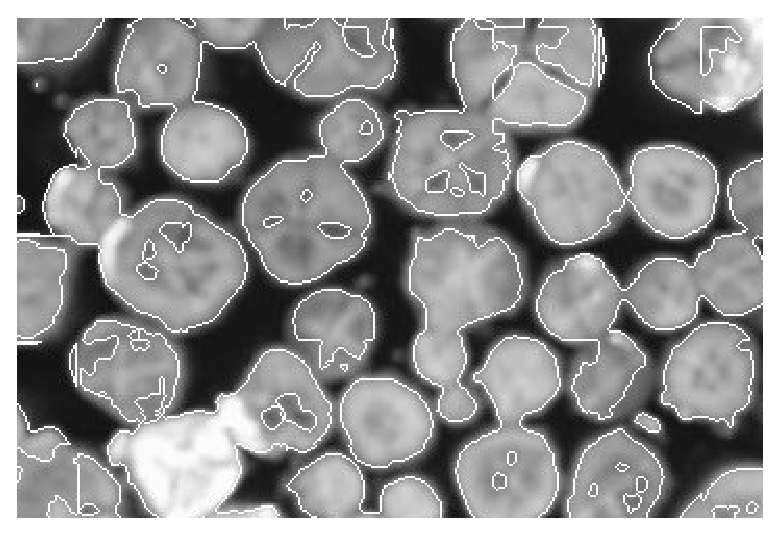
\includegraphics[width=0.7\linewidth]{./images/resultados/fig_me_p1_50x50.eps}
				\par Pilha 1
			\end{center}
		\end{minipage}
		\begin{minipage}[b]{0.45\linewidth}
			\begin{center}
				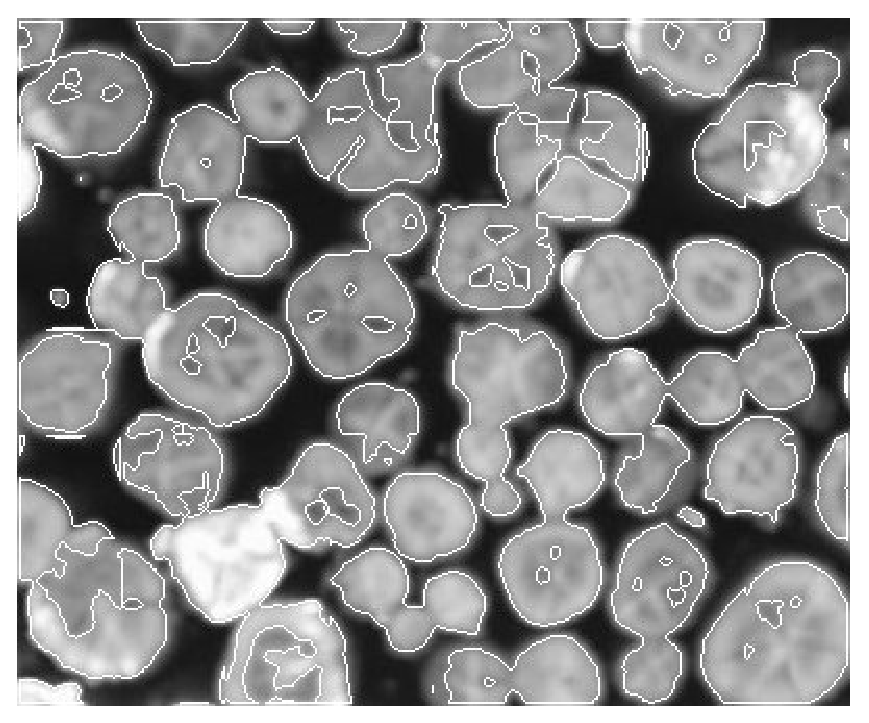
\includegraphics[width=0.7\linewidth]{./images/resultados/fig_me_p2_50x50.eps}
				\par Pilha 2
			\end{center}
		\end{minipage}
		\begin{minipage}[b]{0.45\linewidth}
			\begin{center}
				
\includegraphics[width=0.7\linewidth]{./images/resultados/fig_me_p3_50x50.eps}
				\par Pilha 3
			\end{center}
		\end{minipage}
		\begin{minipage}[b]{0.45\linewidth}
			\begin{center}
				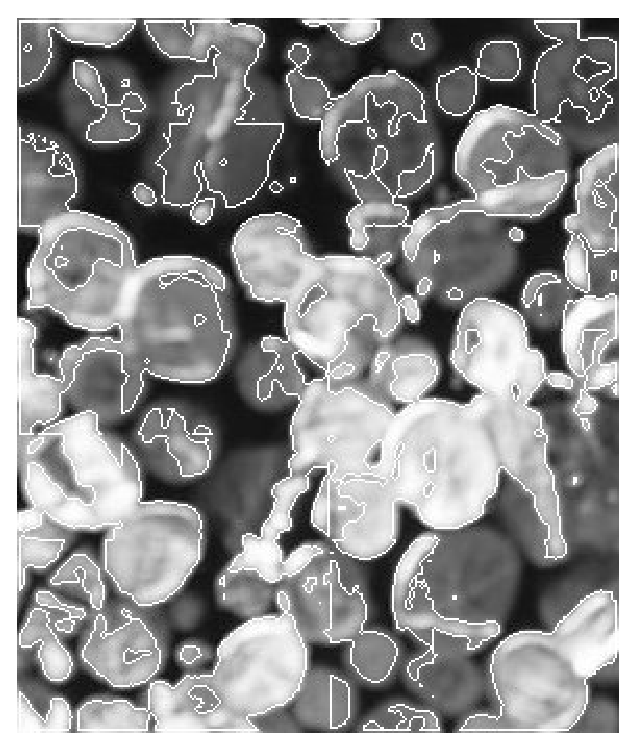
\includegraphics[width=0.7\linewidth]{./images/resultados/fig_me_p4_50x50.eps}
				\par Pilha 4
			\end{center}
		\end{minipage}
		\begin{minipage}[b]{0.45\linewidth}
			\begin{center}
				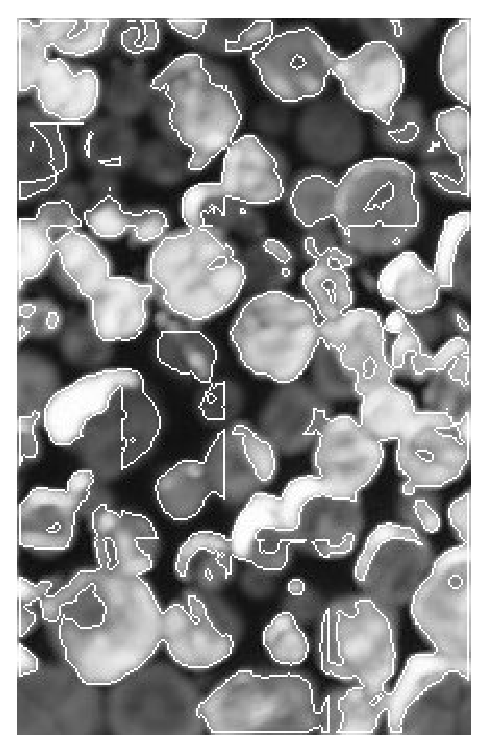
\includegraphics[width=0.7\linewidth]{./images/resultados/fig_me_p5_50x50.eps}
				\par Pilha 5
			\end{center}
		\end{minipage}
	\end{center}
	\par
	\vspace{-0.3cm} \caption{Fotos de resultados obtidos na segmenta��o por m�dia, com janela 50x50 pixels.}
	\label{fig:resultados_media_50x50}
\end{figure}

\begin{figure}[htbp]
	\begin{center}
		\begin{minipage}[b]{0.45\linewidth}
			\begin{center}
				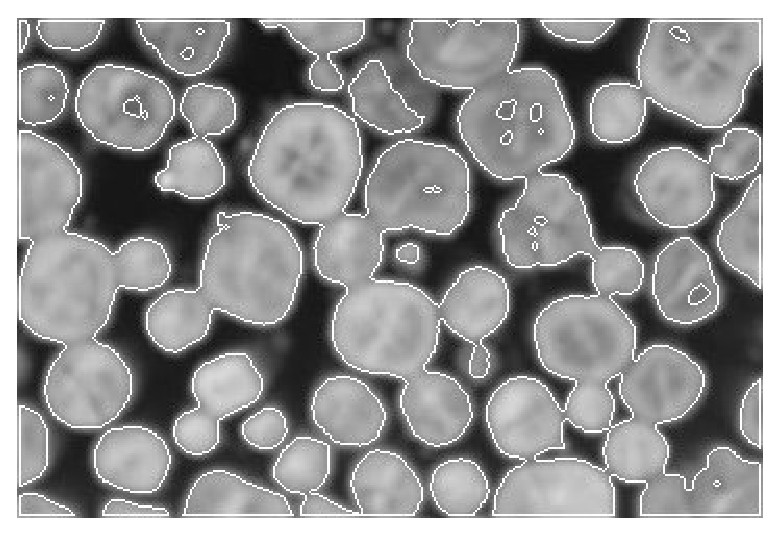
\includegraphics[width=0.7\linewidth]{./images/resultados/fig_me_p1_100x100.eps}
				\par Pilha 1
			\end{center}
		\end{minipage}
		\begin{minipage}[b]{0.45\linewidth}
			\begin{center}
				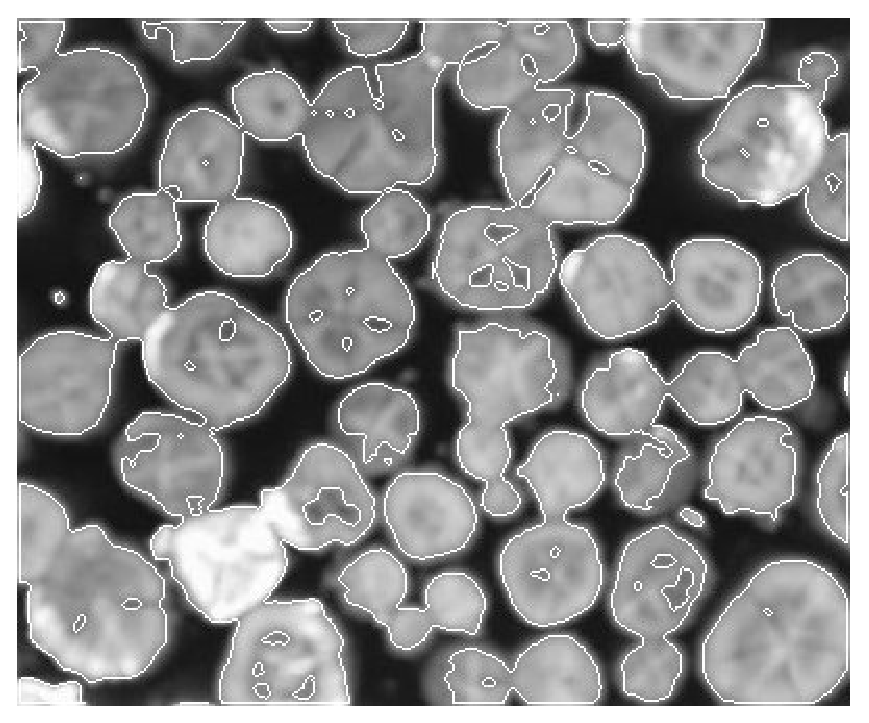
\includegraphics[width=0.7\linewidth]{./images/resultados/fig_me_p2_100x100.eps}
				\par Pilha 2
			\end{center}
		\end{minipage}
		\begin{minipage}[b]{0.45\linewidth}
			\begin{center}
				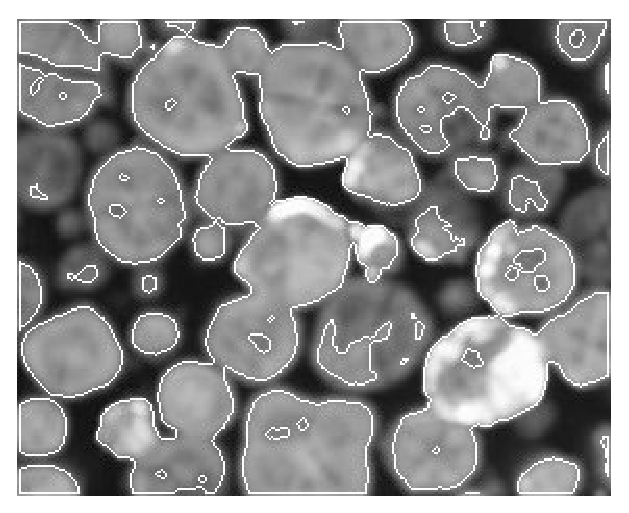
\includegraphics[width=0.7\linewidth]{./images/resultados/fig_me_p3_100x100.eps}
				\par Pilha 3
			\end{center}
		\end{minipage}
		\begin{minipage}[b]{0.45\linewidth}
			\begin{center}
				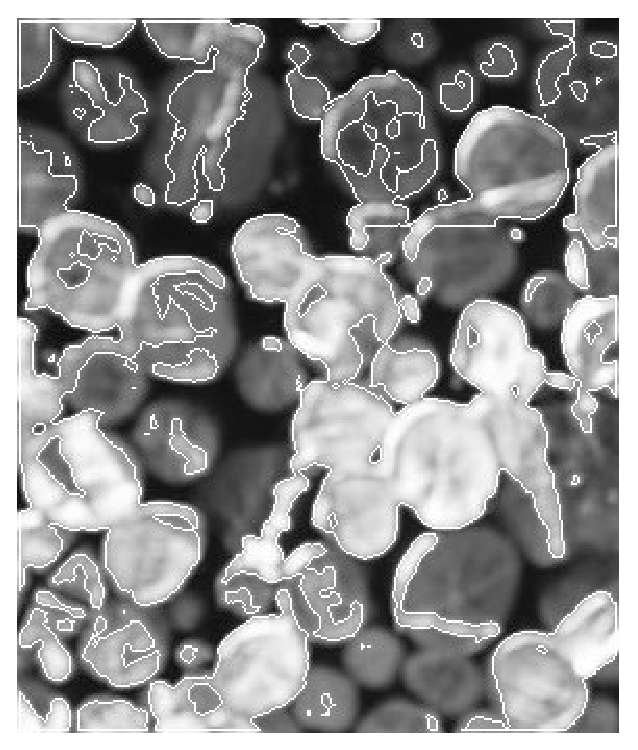
\includegraphics[width=0.7\linewidth]{./images/resultados/fig_me_p4_100x100.eps}
				\par Pilha 4
			\end{center}
		\end{minipage}
		\begin{minipage}[b]{0.45\linewidth}
			\begin{center}
				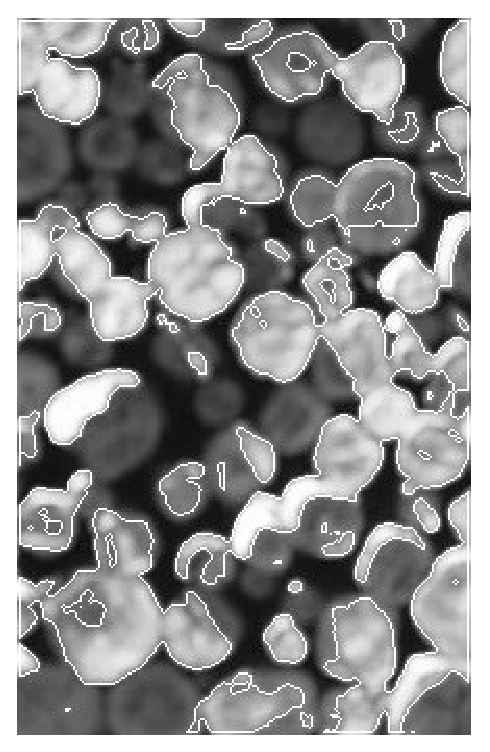
\includegraphics[width=0.7\linewidth]{./images/resultados/fig_me_p5_100x100.eps}
				\par Pilha 5
			\end{center}
		\end{minipage}
	\end{center}
	\par
	\vspace{-0.3cm} \caption{Fotos de resultados obtidos na segmenta��o por m�dia, com janela 100x100 pixels.}
	\label{fig:resultados_media_100x100}
\end{figure}

\begin{figure}[htbp]
	\begin{center}
		\begin{minipage}[b]{0.45\linewidth}
			\begin{center}
				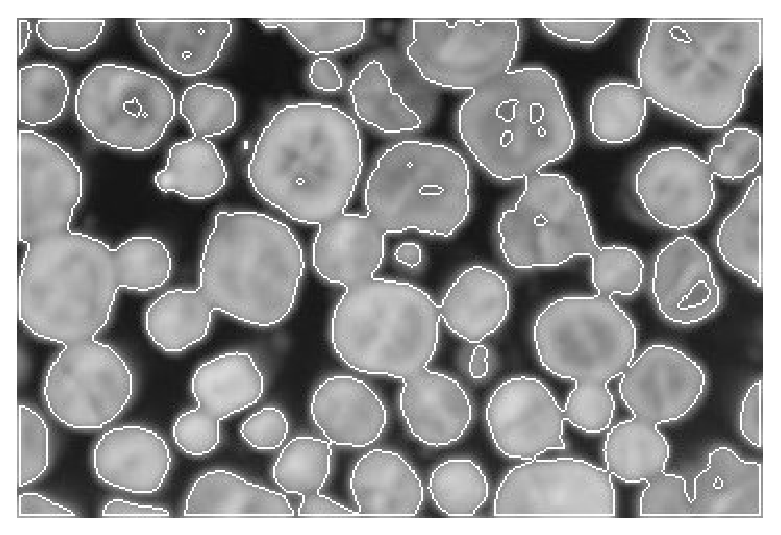
\includegraphics[width=0.7\linewidth]{./images/resultados/fig_me_p1_120x120.eps}
				\par Pilha 1
			\end{center}
		\end{minipage}
		\begin{minipage}[b]{0.45\linewidth}
			\begin{center}
				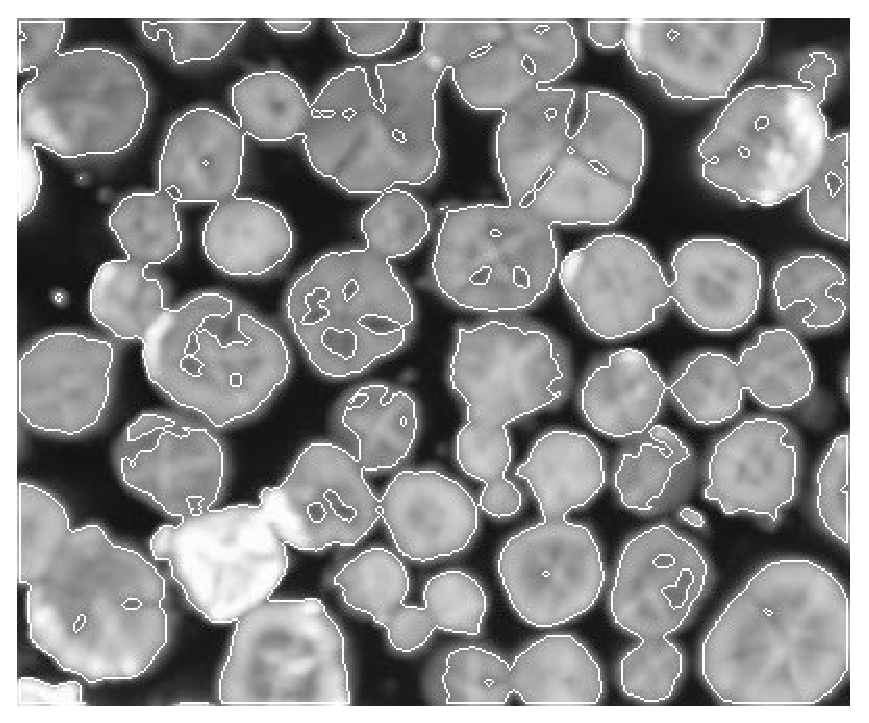
\includegraphics[width=0.7\linewidth]{./images/resultados/fig_me_p2_120x120.eps}
				\par Pilha 2
			\end{center}
		\end{minipage}
		\begin{minipage}[b]{0.45\linewidth}
			\begin{center}
				
\includegraphics[width=0.7\linewidth]{./images/resultados/fig_me_p3_120x120.eps}
				\par Pilha 3
			\end{center}
		\end{minipage}
		\begin{minipage}[b]{0.45\linewidth}
			\begin{center}
				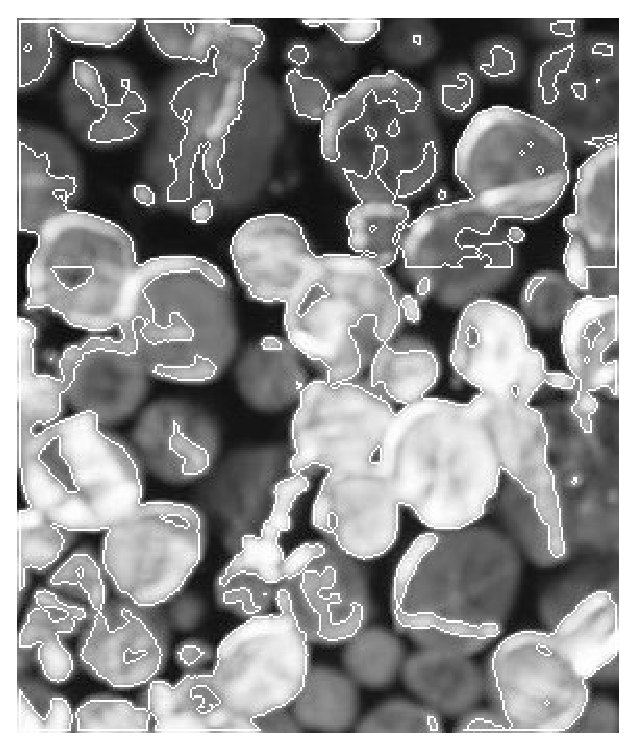
\includegraphics[width=0.7\linewidth]{./images/resultados/fig_me_p4_120x120.eps}
				\par Pilha 4
			\end{center}
		\end{minipage}
		\begin{minipage}[b]{0.45\linewidth}
			\begin{center}
				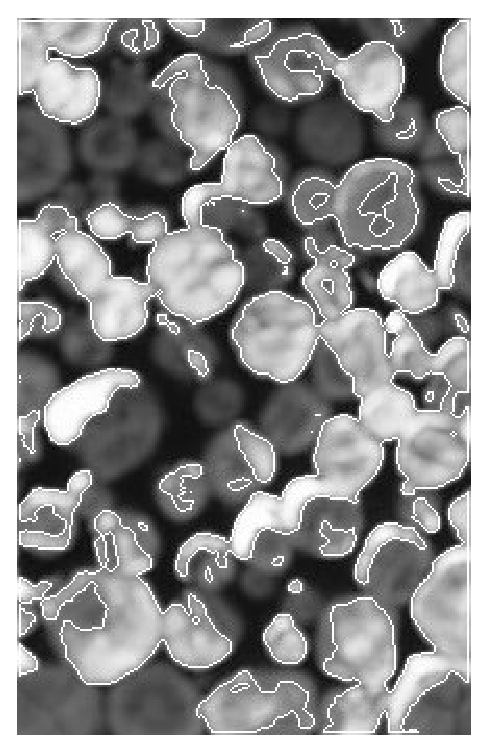
\includegraphics[width=0.7\linewidth]{./images/resultados/fig_me_p5_120x120.eps}
				\par Pilha 5
			\end{center}
		\end{minipage}
	\end{center}
	\par
	\vspace{-0.3cm} \caption{Fotos de resultados obtidos na segmenta��o por m�dia, com janela 120x120 pixels.}
	\label{fig:resultados_media_120x120}
\end{figure}

\begin{figure}[htbp]
	\begin{center}
		\begin{minipage}[b]{0.45\linewidth}
			\begin{center}
				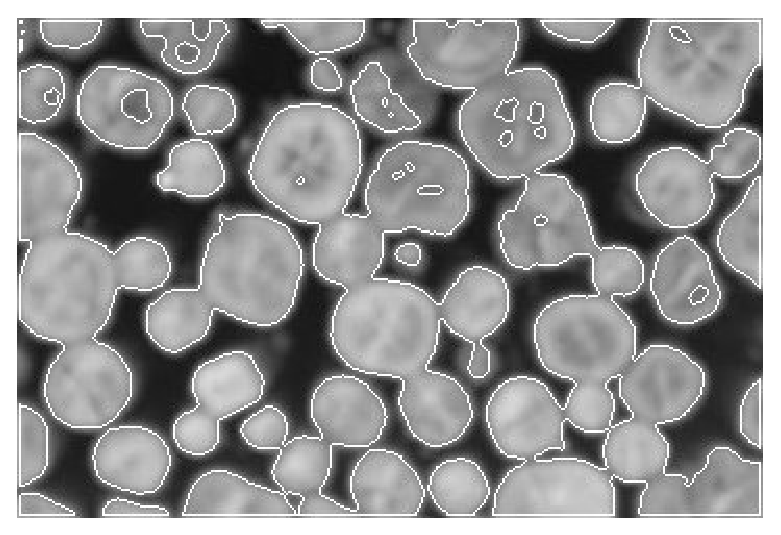
\includegraphics[width=0.7\linewidth]{./images/resultados/fig_me_p1_200x200.eps}
				\par Pilha 1
			\end{center}
		\end{minipage}
		\begin{minipage}[b]{0.45\linewidth}
			\begin{center}
				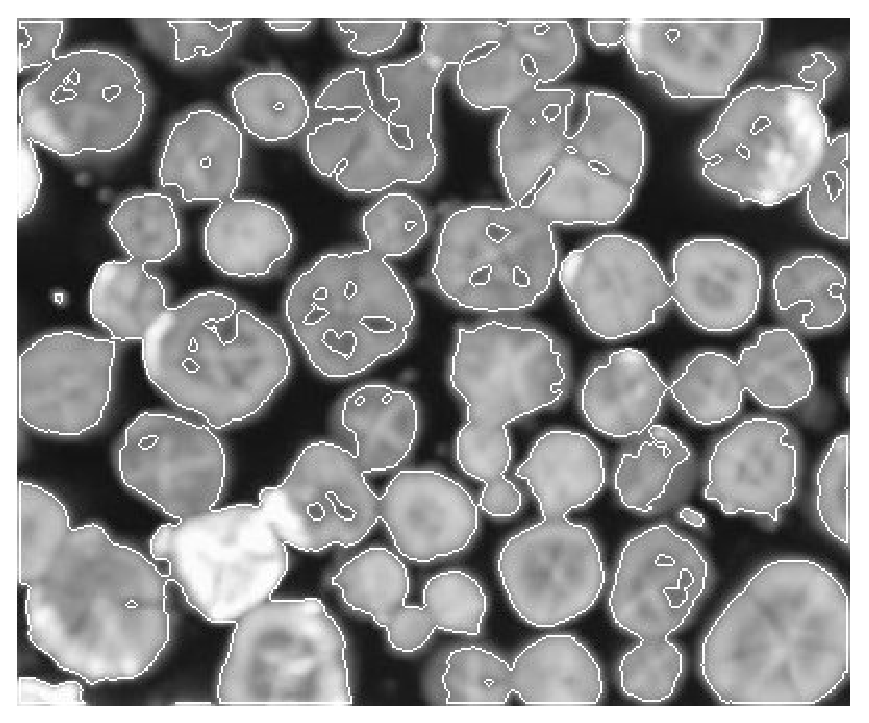
\includegraphics[width=0.7\linewidth]{./images/resultados/fig_me_p2_200x200.eps}
				\par Pilha 2
			\end{center}
		\end{minipage}
		\begin{minipage}[b]{0.45\linewidth}
			\begin{center}
				
\includegraphics[width=0.7\linewidth]{./images/resultados/fig_me_p3_200x200.eps}
				\par Pilha 3
			\end{center}
		\end{minipage}
		\begin{minipage}[b]{0.45\linewidth}
			\begin{center}
				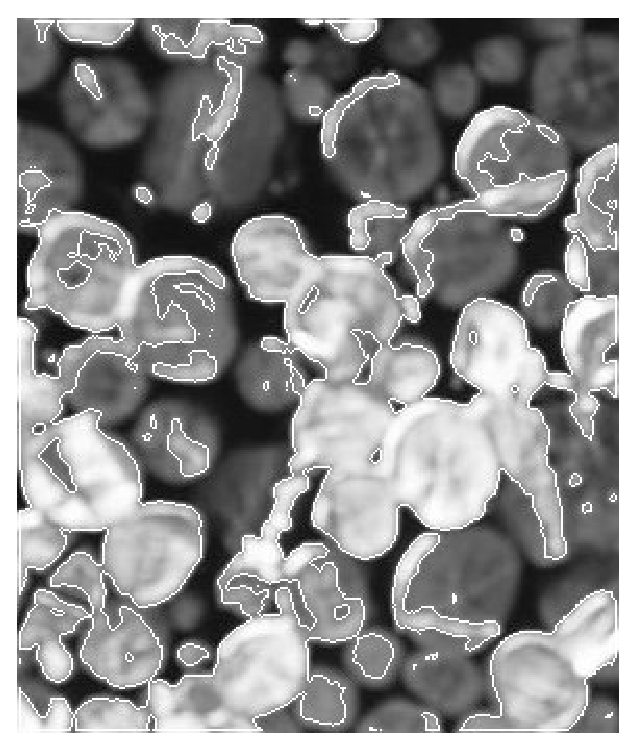
\includegraphics[width=0.7\linewidth]{./images/resultados/fig_me_p4_200x200.eps}
				\par Pilha 4
			\end{center}
		\end{minipage}
		\begin{minipage}[b]{0.45\linewidth}
			\begin{center}
				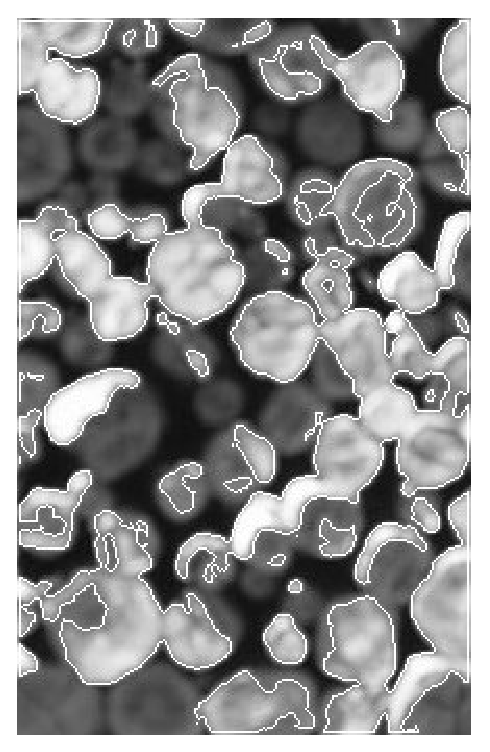
\includegraphics[width=0.7\linewidth]{./images/resultados/fig_me_p5_200x200.eps}
				\par Pilha 5
			\end{center}
		\end{minipage}
	\end{center}
	\par
	\vspace{-0.3cm} \caption{Fotos de resultados obtidos na segmenta��o por m�dia, com janela 200x200 pixels.}
	\label{fig:resultados_media_200x200}
\end{figure}

%Limiar adaptativo

\begin{figure}[htbp]
	\begin{center}
		\begin{minipage}[b]{0.45\linewidth}
			\begin{center}
				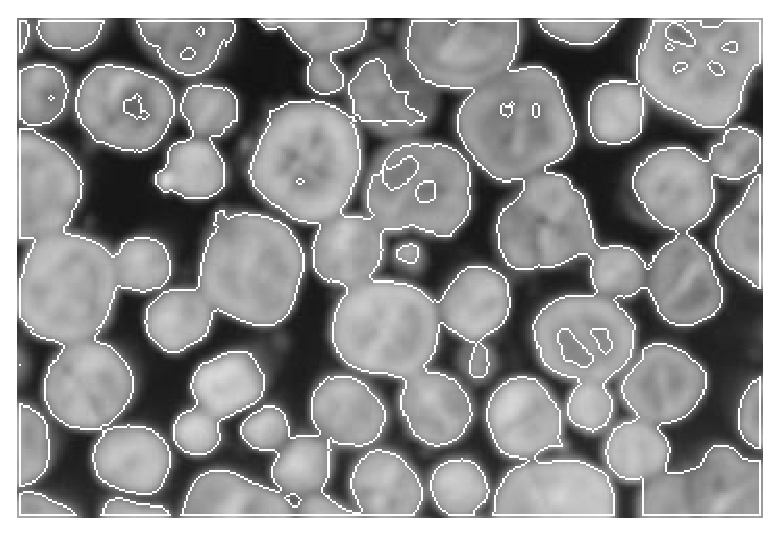
\includegraphics[width=0.7\linewidth]{./images/resultados/fig_la_p1_50x50.eps}
				\par Pilha 1
			\end{center}
		\end{minipage}
		\begin{minipage}[b]{0.45\linewidth}
			\begin{center}
				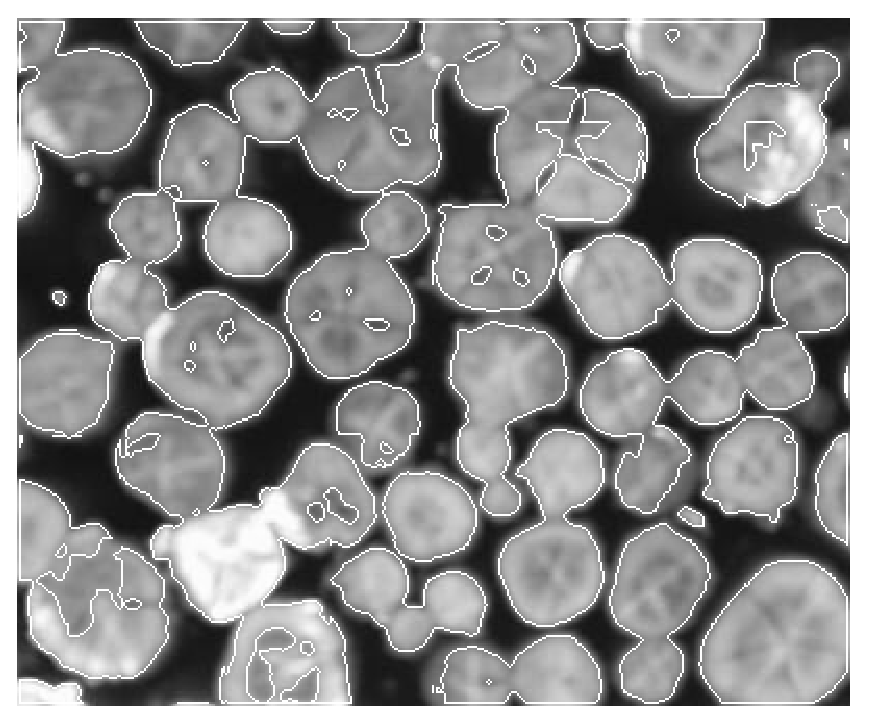
\includegraphics[width=0.7\linewidth]{./images/resultados/fig_la_p2_50x50.eps}
				\par Pilha 2
			\end{center}
		\end{minipage}
		\begin{minipage}[b]{0.45\linewidth}
			\begin{center}
				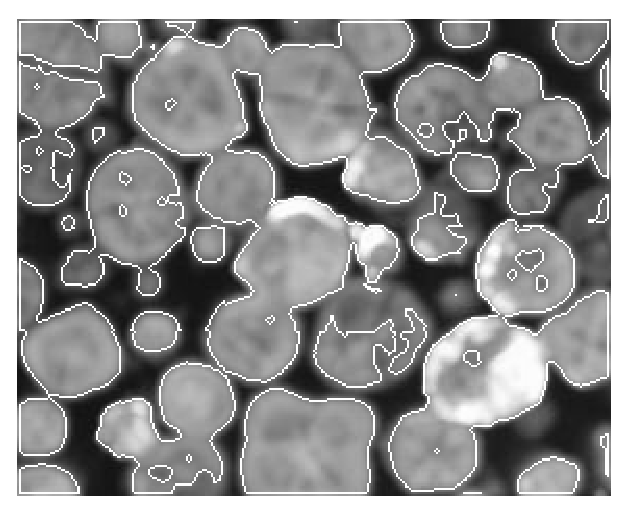
\includegraphics[width=0.7\linewidth]{./images/resultados/fig_la_p3_50x50.eps}
				\par Pilha 3
			\end{center}
		\end{minipage}
		\begin{minipage}[b]{0.45\linewidth}
			\begin{center}
				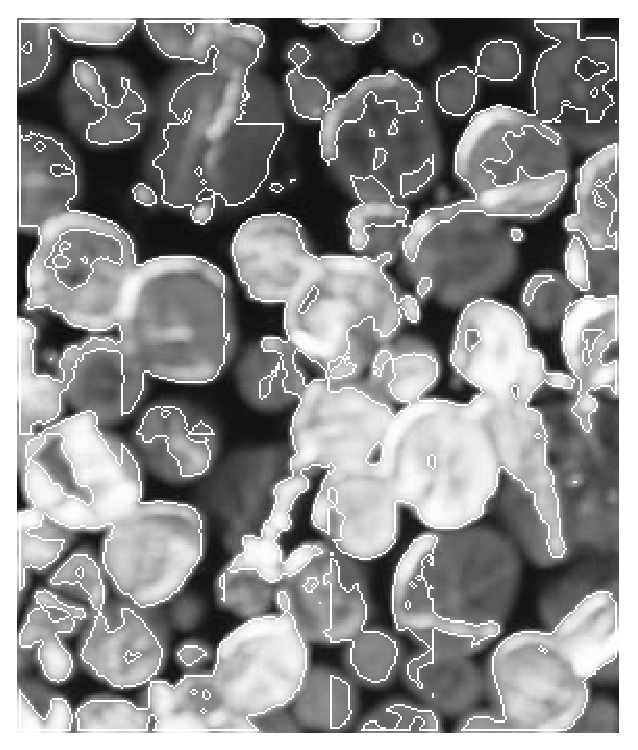
\includegraphics[width=0.7\linewidth]{./images/resultados/fig_la_p4_50x50.eps}
				\par Pilha 4
			\end{center}
		\end{minipage}
		\begin{minipage}[b]{0.45\linewidth}
			\begin{center}
				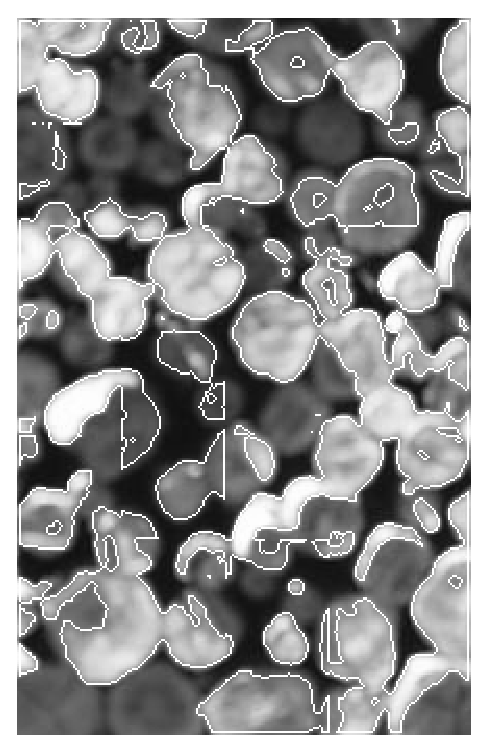
\includegraphics[width=0.7\linewidth]{./images/resultados/fig_la_p5_50x50.eps}
				\par Pilha 5
			\end{center}
		\end{minipage}
	\end{center}
	\par
	\vspace{-0.3cm} \caption{Fotos de resultados obtidos na segmenta��o por limiar adaptativo, com janela 50x50 pixels.}
	\label{fig:resultados_limiar_adaptativo_50x50}
\end{figure}

\begin{figure}[htbp]
	\begin{center}
		\begin{minipage}[b]{0.45\linewidth}
			\begin{center}
				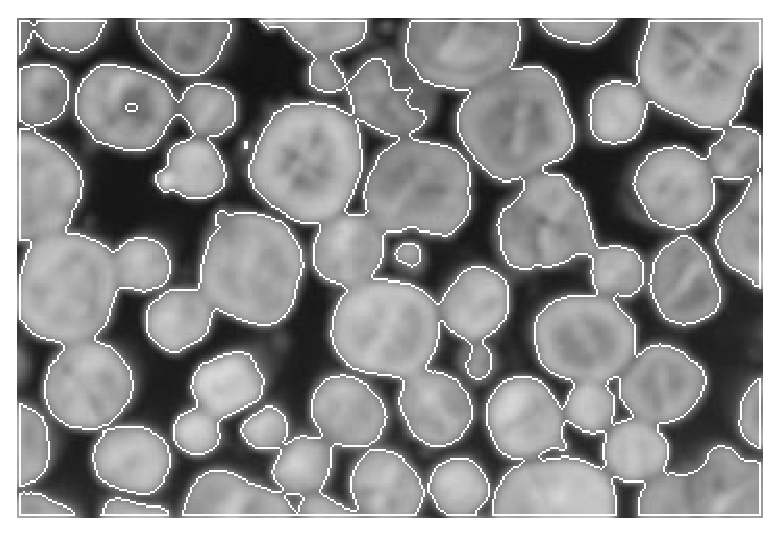
\includegraphics[width=0.7\linewidth]{./images/resultados/fig_la_p1_100x100.eps}
				\par Pilha 1
			\end{center}
		\end{minipage}
		\begin{minipage}[b]{0.45\linewidth}
			\begin{center}
				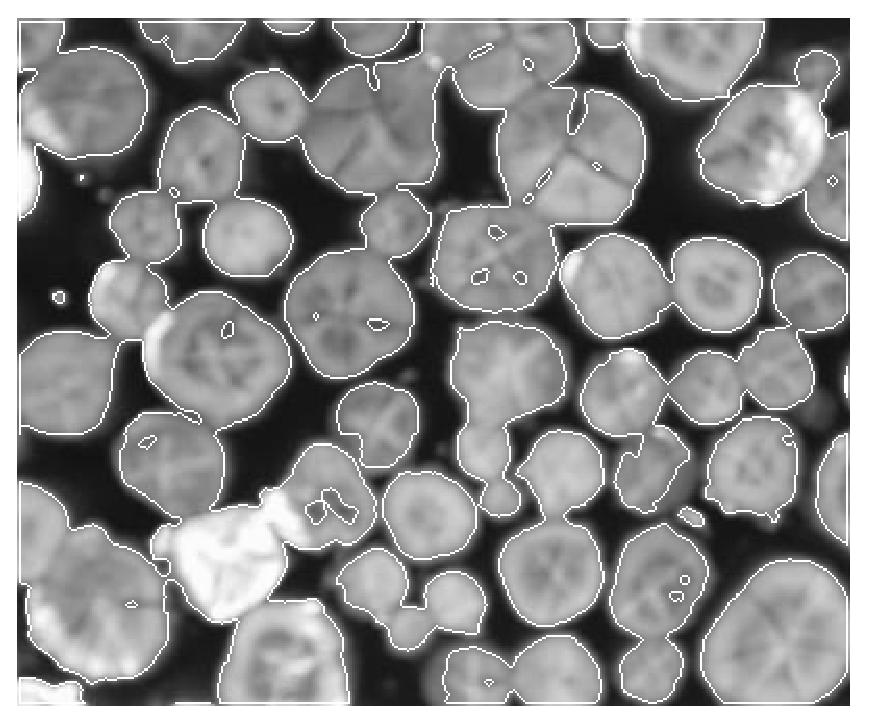
\includegraphics[width=0.7\linewidth]{./images/resultados/fig_la_p2_100x100.eps}
				\par Pilha 2
			\end{center}
		\end{minipage}
		\begin{minipage}[b]{0.45\linewidth}
			\begin{center}
				
\includegraphics[width=0.7\linewidth]{./images/resultados/fig_la_p3_100x100.eps}
				\par Pilha 3
			\end{center}
		\end{minipage}
		\begin{minipage}[b]{0.45\linewidth}
			\begin{center}
				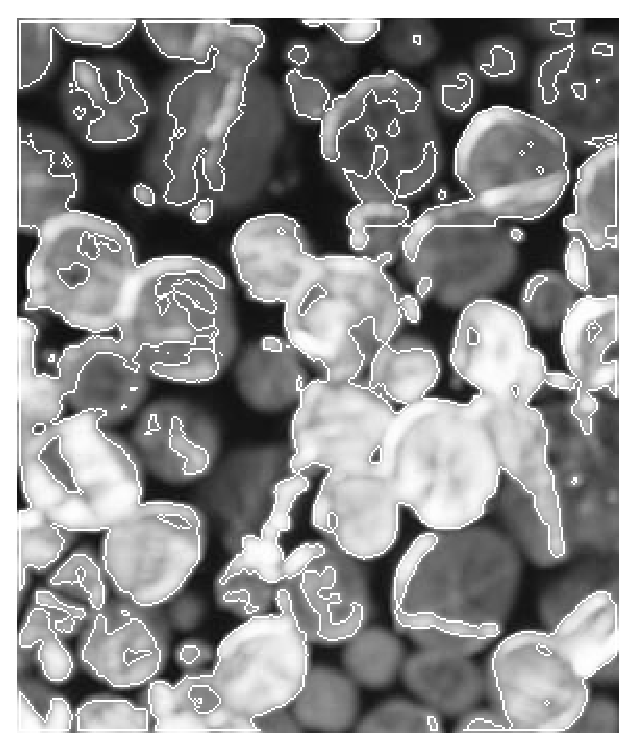
\includegraphics[width=0.7\linewidth]{./images/resultados/fig_la_p4_100x100.eps}
				\par Pilha 4
			\end{center}
		\end{minipage}
		\begin{minipage}[b]{0.45\linewidth}
			\begin{center}
				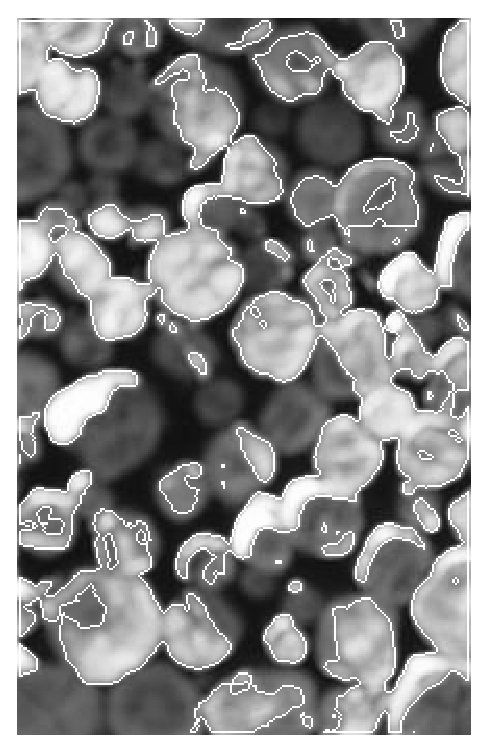
\includegraphics[width=0.7\linewidth]{./images/resultados/fig_la_p5_100x100.eps}
				\par Pilha 5
			\end{center}
		\end{minipage}
	\end{center}
	\par
	\vspace{-0.3cm} \caption{Fotos de resultados obtidos na segmenta��o por limiar adaptativo, com janela 100x100 pixels.}
	\label{fig:resultados_limiar_adaptativo_100x100}
\end{figure}

\begin{figure}[htbp]
	\begin{center}
		\begin{minipage}[b]{0.45\linewidth}
			\begin{center}
				\includegraphics[width=0.7\linewidth]{./images/resultados/fig_la_p1_120x120.eps}
				\par Pilha 1
			\end{center}
		\end{minipage}
		\begin{minipage}[b]{0.45\linewidth}
			\begin{center}
				\includegraphics[width=0.7\linewidth]{./images/resultados/fig_la_p2_120x120.eps}
				\par Pilha 2
			\end{center}
		\end{minipage}
		\begin{minipage}[b]{0.45\linewidth}
			\begin{center}
				\includegraphics[width=0.7\linewidth]{./images/resultados/fig_la_p3_120x120.eps}
				\par Pilha 3
			\end{center}
		\end{minipage}
		\begin{minipage}[b]{0.45\linewidth}
			\begin{center}
				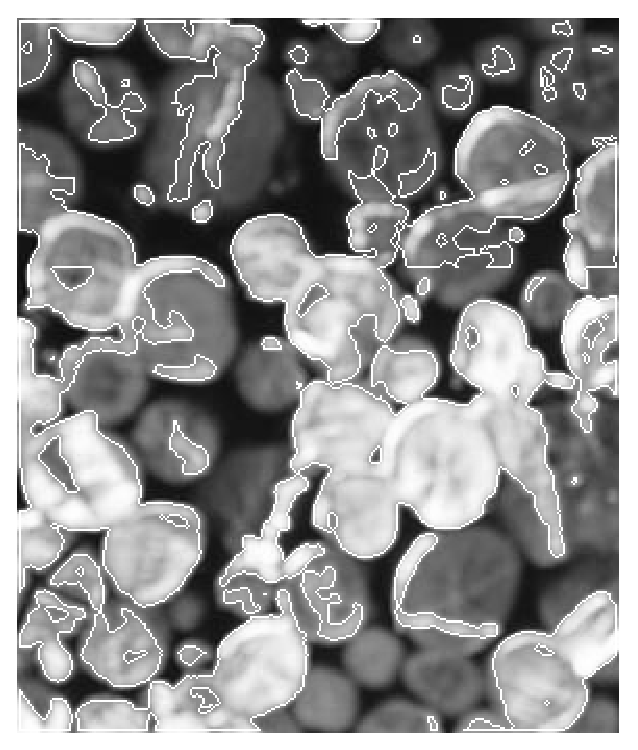
\includegraphics[width=0.7\linewidth]{./images/resultados/fig_la_p4_120x120.eps}
				\par Pilha 4
			\end{center}
		\end{minipage}
		\begin{minipage}[b]{0.45\linewidth}
			\begin{center}
				\includegraphics[width=0.7\linewidth]{./images/resultados/fig_la_p5_120x120.eps}
				\par Pilha 5
			\end{center}
		\end{minipage}
	\end{center}
	\par
	\vspace{-0.3cm} \caption{Fotos de resultados obtidos na segmenta��o por limiar adaptativo, com janela 120x120 pixels.}
	\label{fig:resultados_limiar_adaptativo_120x120}
\end{figure}

\begin{figure}[htbp]
	\begin{center}
		\begin{minipage}[b]{0.45\linewidth}
			\begin{center}
				\includegraphics[width=0.7\linewidth]{./images/resultados/fig_la_p1_200x200.eps}
				\par Pilha 1
			\end{center}
		\end{minipage}
		\begin{minipage}[b]{0.45\linewidth}
			\begin{center}
				\includegraphics[width=0.7\linewidth]{./images/resultados/fig_la_p2_200x200.eps}
				\par Pilha 2
			\end{center}
		\end{minipage}
		\begin{minipage}[b]{0.45\linewidth}
			\begin{center}
				\includegraphics[width=0.7\linewidth]{./images/resultados/fig_la_p3_200x200.eps}
				\par Pilha 3
			\end{center}
		\end{minipage}
		\begin{minipage}[b]{0.45\linewidth}
			\begin{center}
				\includegraphics[width=0.7\linewidth]{./images/resultados/fig_la_p4_200x200.eps}
				\par Pilha 4
			\end{center}
		\end{minipage}
		\begin{minipage}[b]{0.45\linewidth}
			\begin{center}
				\includegraphics[width=0.7\linewidth]{./images/resultados/fig_la_p5_200x200.eps}
				\par Pilha 5
			\end{center}
		\end{minipage}
	\end{center}
	\par
	\vspace{-0.3cm} \caption{Fotos de resultados obtidos na segmenta��o por limiar adaptativo, com janela 200x200 pixels.}
	\label{fig:resultados_limiar_adaptativo_200x200}
\end{figure}

% Shannon
\begin{figure}[htbp]
	\begin{center}
		\begin{minipage}[b]{0.45\linewidth}
			\begin{center}
				\includegraphics[width=0.7\linewidth]{./images/resultados/fig_sh_p1_50x50.eps}
				\par Pilha 1
			\end{center}
		\end{minipage}
		\begin{minipage}[b]{0.45\linewidth}
			\begin{center}
				\includegraphics[width=0.7\linewidth]{./images/resultados/fig_sh_p2_50x50.eps}
				\par Pilha 2
			\end{center}
		\end{minipage}
		\begin{minipage}[b]{0.45\linewidth}
			\begin{center}
				\includegraphics[width=0.7\linewidth]{./images/resultados/fig_sh_p3_50x50.eps}
				\par Pilha 3
			\end{center}
		\end{minipage}
		\begin{minipage}[b]{0.45\linewidth}
			\begin{center}
				\includegraphics[width=0.7\linewidth]{./images/resultados/fig_sh_p4_50x50.eps}
				\par Pilha 4
			\end{center}
		\end{minipage}
		\begin{minipage}[b]{0.45\linewidth}
			\begin{center}
				\includegraphics[width=0.7\linewidth]{./images/resultados/fig_sh_p5_50x50.eps}
				\par Pilha 5
			\end{center}
		\end{minipage}
	\end{center}
	\par
	\vspace{-0.3cm} \caption{Fotos de resultados obtidos na segmenta��o por Entropia de Shannon, com janela 50x50 pixels.}
	\label{fig:resultados_entropia_shannon_50x50}
\end{figure}

\begin{figure}[htbp]
	\begin{center}
		\begin{minipage}[b]{0.45\linewidth}
			\begin{center}
				\includegraphics[width=0.7\linewidth]{./images/resultados/fig_sh_p1_100x100.eps}
				\par Pilha 1
			\end{center}
		\end{minipage}
		\begin{minipage}[b]{0.45\linewidth}
			\begin{center}
				\includegraphics[width=0.7\linewidth]{./images/resultados/fig_sh_p2_100x100.eps}
				\par Pilha 2
			\end{center}
		\end{minipage}
		\begin{minipage}[b]{0.45\linewidth}
			\begin{center}
				\includegraphics[width=0.7\linewidth]{./images/resultados/fig_sh_p3_100x100.eps}
				\par Pilha 3
			\end{center}
		\end{minipage}
		\begin{minipage}[b]{0.45\linewidth}
			\begin{center}
				\includegraphics[width=0.7\linewidth]{./images/resultados/fig_sh_p4_100x100.eps}
				\par Pilha 4
			\end{center}
		\end{minipage}
		\begin{minipage}[b]{0.45\linewidth}
			\begin{center}
				\includegraphics[width=0.7\linewidth]{./images/resultados/fig_sh_p5_100x100.eps}
				\par Pilha 5
			\end{center}
		\end{minipage}
	\end{center}
	\par
	\vspace{-0.3cm} \caption{Fotos de resultados obtidos na segmenta��o por Entropia de Shannon, com janela 100x100 pixels.}
	\label{fig:resultados_entropia_shannon_100x100}
\end{figure}

\begin{figure}[htbp]
	\begin{center}
		\begin{minipage}[b]{0.45\linewidth}
			\begin{center}
				\includegraphics[width=0.7\linewidth]{./images/resultados/fig_sh_p1_120x120.eps}
				\par Pilha 1
			\end{center}
		\end{minipage}
		\begin{minipage}[b]{0.45\linewidth}
			\begin{center}
				\includegraphics[width=0.7\linewidth]{./images/resultados/fig_sh_p2_120x120.eps}
				\par Pilha 2
			\end{center}
		\end{minipage}
		\begin{minipage}[b]{0.45\linewidth}
			\begin{center}
				\includegraphics[width=0.7\linewidth]{./images/resultados/fig_sh_p3_120x120.eps}
				\par Pilha 3
			\end{center}
		\end{minipage}
		\begin{minipage}[b]{0.45\linewidth}
			\begin{center}
				\includegraphics[width=0.7\linewidth]{./images/resultados/fig_sh_p4_120x120.eps}
				\par Pilha 4
			\end{center}
		\end{minipage}
		\begin{minipage}[b]{0.45\linewidth}
			\begin{center}
				\includegraphics[width=0.7\linewidth]{./images/resultados/fig_sh_p5_120x120.eps}
				\par Pilha 5
			\end{center}
		\end{minipage}
	\end{center}
	\par
	\vspace{-0.3cm} \caption{Fotos de resultados obtidos na segmenta��o por Entropia de Shannon, com janela 120x120 pixels.}
	\label{fig:resultados_entropia_shannon_120x120}
\end{figure}

\begin{figure}[htbp]
	\begin{center}
		\begin{minipage}[b]{0.45\linewidth}
			\begin{center}
				\includegraphics[width=0.7\linewidth]{./images/resultados/fig_sh_p1_200x200.eps}
				\par Pilha 1
			\end{center}
		\end{minipage}
		\begin{minipage}[b]{0.45\linewidth}
			\begin{center}
				\includegraphics[width=0.7\linewidth]{./images/resultados/fig_sh_p2_200x200.eps}
				\par Pilha 2
			\end{center}
		\end{minipage}
		\begin{minipage}[b]{0.45\linewidth}
			\begin{center}
				\includegraphics[width=0.7\linewidth]{./images/resultados/fig_sh_p3_200x200.eps}
				\par Pilha 3
			\end{center}
		\end{minipage}
		\begin{minipage}[b]{0.45\linewidth}
			\begin{center}
				\includegraphics[width=0.7\linewidth]{./images/resultados/fig_sh_p4_200x200.eps}
				\par Pilha 4
			\end{center}
		\end{minipage}
		\begin{minipage}[b]{0.45\linewidth}
			\begin{center}
				\includegraphics[width=0.7\linewidth]{./images/resultados/fig_sh_p5_200x200.eps}
				\par Pilha 5
			\end{center}
		\end{minipage}
	\end{center}
	\par
	\vspace{-0.3cm} \caption{Fotos de resultados obtidos na segmenta��o por Entropia de Shannon, com janela 200x200 pixels.}
	\label{fig:resultados_entropia_shannon_200x200}
\end{figure}

%q=-2.0

\begin{figure}[htbp]
	\begin{center}
		\begin{minipage}[b]{0.45\linewidth}
			\begin{center}
				\includegraphics[width=0.7\linewidth]{./images/resultados/fig_ts_p1_50x50_q-2.0.eps}
				\par Pilha 1
			\end{center}
		\end{minipage}
		\begin{minipage}[b]{0.45\linewidth}
			\begin{center}
				\includegraphics[width=0.7\linewidth]{./images/resultados/fig_ts_p2_50x50_q-2.0.eps}
				\par Pilha 2
			\end{center}
		\end{minipage}
		\begin{minipage}[b]{0.45\linewidth}
			\begin{center}
				\includegraphics[width=0.7\linewidth]{./images/resultados/fig_ts_p3_50x50_q-2.0.eps}
				\par Pilha 3
			\end{center}
		\end{minipage}
		\begin{minipage}[b]{0.45\linewidth}
			\begin{center}
				\includegraphics[width=0.7\linewidth]{./images/resultados/fig_ts_p4_50x50_q-2.0.eps}
				\par Pilha 4
			\end{center}
		\end{minipage}
		\begin{minipage}[b]{0.45\linewidth}
			\begin{center}
				\includegraphics[width=0.7\linewidth]{./images/resultados/fig_ts_p5_50x50_q-2.0.eps}
				\par Pilha 5
			\end{center}
		\end{minipage}
	\end{center}
	\par
	\vspace{-0.3cm} \caption{Fotos de resultados obtidos na segmenta��o por Entropia de Tsallis, com $q=-2.0$ e janela 50x50 pixels.}
	\label{fig:resultados_entropia_tsallis_q_-20_50x50}
\end{figure}

\begin{figure}[htbp]
	\begin{center}
		\begin{minipage}[b]{0.45\linewidth}
			\begin{center}
				\includegraphics[width=0.7\linewidth]{./images/resultados/fig_ts_p1_100x100_q-2.0.eps}
				\par Pilha 1
			\end{center}
		\end{minipage}
		\begin{minipage}[b]{0.45\linewidth}
			\begin{center}
				\includegraphics[width=0.7\linewidth]{./images/resultados/fig_ts_p2_100x100_q-2.0.eps}
				\par Pilha 2
			\end{center}
		\end{minipage}
		\begin{minipage}[b]{0.45\linewidth}
			\begin{center}
				\includegraphics[width=0.7\linewidth]{./images/resultados/fig_ts_p3_100x100_q-2.0.eps}
				\par Pilha 3
			\end{center}
		\end{minipage}
		\begin{minipage}[b]{0.45\linewidth}
			\begin{center}
				\includegraphics[width=0.7\linewidth]{./images/resultados/fig_ts_p4_100x100_q-2.0.eps}
				\par Pilha 4
			\end{center}
		\end{minipage}
		\begin{minipage}[b]{0.45\linewidth}
			\begin{center}
				\includegraphics[width=0.7\linewidth]{./images/resultados/fig_ts_p5_100x100_q-2.0.eps}
				\par Pilha 5
			\end{center}
		\end{minipage}
	\end{center}
	\par
	\vspace{-0.3cm} \caption{Fotos de resultados obtidos na segmenta��o por Entropia de Tsallis,  com $q=-2.0$ e janela 100x100 pixels.}
	\label{fig:resultados_entropia_tsallis_q_-20_100x100}
\end{figure}

%q=-1.5

%\begin{figure}[htbp]
%	\begin{center}
%		\begin{minipage}[b]{0.45\linewidth}
%			\begin{center}
%				\includegraphics[width=0.7\linewidth]{./images/resultados/fig_ts_p1_50x50_q-1.5.eps}
%				\par Pilha 1
%			\end{center}
%		\end{minipage}
%		\begin{minipage}[b]{0.45\linewidth}
%			\begin{center}
%				\includegraphics[width=0.7\linewidth]{./images/resultados/fig_ts_p2_50x50_q-1.5.eps}
%				\par Pilha 2
%			\end{center}
%		\end{minipage}
%		\begin{minipage}[b]{0.45\linewidth}
%			\begin{center}
%				\includegraphics[width=0.7\linewidth]{./images/resultados/fig_ts_p3_50x50_q-1.5.eps}
%				\par Pilha 3
%			\end{center}
%		\end{minipage}
%		\begin{minipage}[b]{0.45\linewidth}
%			\begin{center}
%				\includegraphics[width=0.7\linewidth]{./images/resultados/fig_ts_p4_50x50_q-1.5.eps}
%				\par Pilha 4
%			\end{center}
%		\end{minipage}
%		\begin{minipage}[b]{0.45\linewidth}
%			\begin{center}
%				\includegraphics[width=0.7\linewidth]{./images/resultados/fig_ts_p5_50x50_q-1.5.eps}
%				\par Pilha 5
%			\end{center}
%		\end{minipage}
%	\end{center}
%	\par
%	\vspace{-0.3cm} \caption{Fotos de resultados obtidos na segmenta��o por Entropia de tsallis, com $q=-1,5$ e janela 50x50 pixels.}
%	\label{fig:resultados_entropia_tsallis_q_-15_50x50}
%\end{figure}
%
%\begin{figure}[htbp]
%	\begin{center}
%		\begin{minipage}[b]{0.45\linewidth}
%			\begin{center}
%				\includegraphics[width=0.7\linewidth]{./images/resultados/fig_ts_p1_100x100_q-1.5.eps}
%				\par Pilha 1
%			\end{center}
%		\end{minipage}
%		\begin{minipage}[b]{0.45\linewidth}
%			\begin{center}
%				\includegraphics[width=0.7\linewidth]{./images/resultados/fig_ts_p2_100x100_q-1.5.eps}
%				\par Pilha 2
%			\end{center}
%		\end{minipage}
%		\begin{minipage}[b]{0.45\linewidth}
%			\begin{center}
%				\includegraphics[width=0.7\linewidth]{./images/resultados/fig_ts_p3_100x100_q-1.5.eps}
%				\par Pilha 3
%			\end{center}
%		\end{minipage}
%		\begin{minipage}[b]{0.45\linewidth}
%			\begin{center}
%				\includegraphics[width=0.7\linewidth]{./images/resultados/fig_ts_p4_100x100_q-1.5.eps}
%				\par Pilha 4
%			\end{center}
%		\end{minipage}
%		\begin{minipage}[b]{0.45\linewidth}
%			\begin{center}
%				\includegraphics[width=0.7\linewidth]{./images/resultados/fig_ts_p5_100x100_q-1.5.eps}
%				\par Pilha 5
%			\end{center}
%		\end{minipage}
%	\end{center}
%	\par
%	\vspace{-0.3cm} \caption{Fotos de resultados obtidos na segmenta��o por Entropia de tsallis,  com $q=-1,5$ e janela 100x100 pixels.}
%	\label{fig:resultados_entropia_tsallis_q_-15_100x100}
%\end{figure}

%q=-1

%q=0

%q=0.5

%\begin{figure}[htbp]
%	\begin{center}
%		\begin{minipage}[b]{0.45\linewidth}
%			\begin{center}
%				\includegraphics[width=0.7\linewidth]{./images/resultados/fig_ts_p1_50x50_q0.5.eps}
%				\par Pilha 1
%			\end{center}
%		\end{minipage}
%		\begin{minipage}[b]{0.45\linewidth}
%			\begin{center}
%				\includegraphics[width=0.7\linewidth]{./images/resultados/fig_ts_p2_50x50_q0.5.eps}
%				\par Pilha 2
%			\end{center}
%		\end{minipage}
%		\begin{minipage}[b]{0.45\linewidth}
%			\begin{center}
%				\includegraphics[width=0.7\linewidth]{./images/resultados/fig_ts_p3_50x50_q0.5.eps}
%				\par Pilha 3
%			\end{center}
%		\end{minipage}
%		\begin{minipage}[b]{0.45\linewidth}
%			\begin{center}
%				\includegraphics[width=0.7\linewidth]{./images/resultados/fig_ts_p4_50x50_q0.5.eps}
%				\par Pilha 4
%			\end{center}
%		\end{minipage}
%		\begin{minipage}[b]{0.45\linewidth}
%			\begin{center}
%				\includegraphics[width=0.7\linewidth]{./images/resultados/fig_ts_p5_50x50_q0.5.eps}
%				\par Pilha 5
%			\end{center}
%		\end{minipage}
%	\end{center}
%	\par
%	\vspace{-0.3cm} \caption{Fotos de resultados obtidos na segmenta��o por Entropia de tsallis, com $q=0.5$ e janela 50x50 pixels.}
%	\label{fig:resultados_entropia_tsallis_q_05_50x50}
%\end{figure}
%
%\begin{figure}[htbp]
%	\begin{center}
%		\begin{minipage}[b]{0.45\linewidth}
%			\begin{center}
%				\includegraphics[width=0.7\linewidth]{./images/resultados/fig_ts_p1_100x100_q0.5.eps}
%				\par Pilha 1
%			\end{center}
%		\end{minipage}
%		\begin{minipage}[b]{0.45\linewidth}
%			\begin{center}
%				\includegraphics[width=0.7\linewidth]{./images/resultados/fig_ts_p2_100x100_q0.5.eps}
%				\par Pilha 2
%			\end{center}
%		\end{minipage}
%		\begin{minipage}[b]{0.45\linewidth}
%			\begin{center}
%				\includegraphics[width=0.7\linewidth]{./images/resultados/fig_ts_p3_100x100_q0.5.eps}
%				\par Pilha 3
%			\end{center}
%		\end{minipage}
%		\begin{minipage}[b]{0.45\linewidth}
%			\begin{center}
%				\includegraphics[width=0.7\linewidth]{./images/resultados/fig_ts_p4_100x100_q0.5.eps}
%				\par Pilha 4
%			\end{center}
%		\end{minipage}
%		\begin{minipage}[b]{0.45\linewidth}
%			\begin{center}
%				\includegraphics[width=0.7\linewidth]{./images/resultados/fig_ts_p5_100x100_q0.5.eps}
%				\par Pilha 5
%			\end{center}
%		\end{minipage}
%	\end{center}
%	\par
%	\vspace{-0.3cm} \caption{Fotos de resultados obtidos na segmenta��o por Entropia de tsallis,  com $q=0.5$ e janela 100x100 pixels.}
%	\label{fig:resultados_entropia_tsallis_q_05_100x100}
%\end{figure}

%q=1.5

%\begin{figure}[htbp]
%	\begin{center}
%		\begin{minipage}[b]{0.45\linewidth}
%			\begin{center}
%				\includegraphics[width=0.7\linewidth]{./images/resultados/fig_ts_p1_50x50_q1.5.eps}
%				\par Pilha 1
%			\end{center}
%		\end{minipage}
%		\begin{minipage}[b]{0.45\linewidth}
%			\begin{center}
%				\includegraphics[width=0.7\linewidth]{./images/resultados/fig_ts_p2_50x50_q1.5.eps}
%				\par Pilha 2
%			\end{center}
%		\end{minipage}
%		\begin{minipage}[b]{0.45\linewidth}
%			\begin{center}
%				\includegraphics[width=0.7\linewidth]{./images/resultados/fig_ts_p3_50x50_q1.5.eps}
%				\par Pilha 3
%			\end{center}
%		\end{minipage}
%		\begin{minipage}[b]{0.45\linewidth}
%			\begin{center}
%				\includegraphics[width=0.7\linewidth]{./images/resultados/fig_ts_p4_50x50_q1.5.eps}
%				\par Pilha 4
%			\end{center}
%		\end{minipage}
%		\begin{minipage}[b]{0.45\linewidth}
%			\begin{center}
%				\includegraphics[width=0.7\linewidth]{./images/resultados/fig_ts_p5_50x50_q1.5.eps}
%				\par Pilha 5
%			\end{center}
%		\end{minipage}
%	\end{center}
%	\par
%	\vspace{-0.3cm} \caption{Fotos de resultados obtidos na segmenta��o por Entropia de tsallis, com $q=1,5$ e janela 50x50 pixels.}
%	\label{fig:resultados_entropia_tsallis_q_15_50x50}
%\end{figure}
%
%\begin{figure}[htbp]
%	\begin{center}
%		\begin{minipage}[b]{0.45\linewidth}
%			\begin{center}
%				\includegraphics[width=0.7\linewidth]{./images/resultados/fig_ts_p1_100x100_q1.5.eps}
%				\par Pilha 1
%			\end{center}
%		\end{minipage}
%		\begin{minipage}[b]{0.45\linewidth}
%			\begin{center}
%				\includegraphics[width=0.7\linewidth]{./images/resultados/fig_ts_p2_100x100_q1.5.eps}
%				\par Pilha 2
%			\end{center}
%		\end{minipage}
%		\begin{minipage}[b]{0.45\linewidth}
%			\begin{center}
%				\includegraphics[width=0.7\linewidth]{./images/resultados/fig_ts_p3_100x100_q1.5.eps}
%				\par Pilha 3
%			\end{center}
%		\end{minipage}
%		\begin{minipage}[b]{0.45\linewidth}
%			\begin{center}
%				\includegraphics[width=0.7\linewidth]{./images/resultados/fig_ts_p4_100x100_q1.5.eps}
%				\par Pilha 4
%			\end{center}
%		\end{minipage}
%		\begin{minipage}[b]{0.45\linewidth}
%			\begin{center}
%				\includegraphics[width=0.7\linewidth]{./images/resultados/fig_ts_p5_100x100_q1.5.eps}
%				\par Pilha 5
%			\end{center}
%		\end{minipage}
%	\end{center}
%	\par
%	\vspace{-0.3cm} \caption{Fotos de resultados obtidos na segmenta��o por Entropia de tsallis,  com $q=1,5$ e janela 100x100 pixels.}
%	\label{fig:resultados_entropia_tsallis_q_15_100x100}
%\end{figure}


%q=2.0

\begin{figure}[htbp]
	\begin{center}
		\begin{minipage}[b]{0.45\linewidth}
			\begin{center}
				\includegraphics[width=0.7\linewidth]{./images/resultados/fig_ts_p1_50x50_q2.0.eps}
				\par Pilha 1
			\end{center}
		\end{minipage}
		\begin{minipage}[b]{0.45\linewidth}
			\begin{center}
				\includegraphics[width=0.7\linewidth]{./images/resultados/fig_ts_p2_50x50_q2.0.eps}
				\par Pilha 2
			\end{center}
		\end{minipage}
		\begin{minipage}[b]{0.45\linewidth}
			\begin{center}
				\includegraphics[width=0.7\linewidth]{./images/resultados/fig_ts_p3_50x50_q2.0.eps}
				\par Pilha 3
			\end{center}
		\end{minipage}
		\begin{minipage}[b]{0.45\linewidth}
			\begin{center}
				\includegraphics[width=0.7\linewidth]{./images/resultados/fig_ts_p4_50x50_q2.0.eps}
				\par Pilha 4
			\end{center}
		\end{minipage}
		\begin{minipage}[b]{0.45\linewidth}
			\begin{center}
				\includegraphics[width=0.7\linewidth]{./images/resultados/fig_ts_p5_50x50_q2.0.eps}
				\par Pilha 5
			\end{center}
		\end{minipage}
	\end{center}
	\par
	\vspace{-0.3cm} \caption{Fotos de resultados obtidos na segmenta��o por Entropia de Tsallis, com $q=2,0$ e janela 50x50 pixels.}
	\label{fig:resultados_entropia_tsallis_q_20_50x50}
\end{figure}

\begin{figure}[htbp]
	\begin{center}
		\begin{minipage}[b]{0.45\linewidth}
			\begin{center}
				\includegraphics[width=0.7\linewidth]{./images/resultados/fig_ts_p1_100x100_q2.0.eps}
				\par Pilha 1
			\end{center}
		\end{minipage}
		\begin{minipage}[b]{0.45\linewidth}
			\begin{center}
				\includegraphics[width=0.7\linewidth]{./images/resultados/fig_ts_p2_100x100_q2.0.eps}
				\par Pilha 2
			\end{center}
		\end{minipage}
		\begin{minipage}[b]{0.45\linewidth}
			\begin{center}
				\includegraphics[width=0.7\linewidth]{./images/resultados/fig_ts_p3_100x100_q2.0.eps}
				\par Pilha 3
			\end{center}
		\end{minipage}
		\begin{minipage}[b]{0.45\linewidth}
			\begin{center}
				\includegraphics[width=0.7\linewidth]{./images/resultados/fig_ts_p4_100x100_q2.0.eps}
				\par Pilha 4
			\end{center}
		\end{minipage}
		\begin{minipage}[b]{0.45\linewidth}
			\begin{center}
				\includegraphics[width=0.7\linewidth]{./images/resultados/fig_ts_p5_100x100_q2.0.eps}
				\par Pilha 5
			\end{center}
		\end{minipage}
	\end{center}
	\par
	\vspace{-0.3cm} \caption{Fotos de resultados obtidos na segmenta��o por Entropia de Tsallis,  com $q=2,0$ e janela 100x100 pixels.}
	\label{fig:resultados_entropia_tsallis_q_20_100x100}
\end{figure}

%%%%%%%%%%%%%%%%%%%%%%%%%%%%%%%%%%%%%
%%   CONCLUS�ES E TRABALHOS FUTUROS
%%%%%%%%%%%%%%%%%%%%%%%%%%%%%%%%%%%%%


\chapter{Conclus�es e Trabalhos Futuros}
\label{cap:conclusao}

\end{spacing}

% Aqui ser� adicionado ao contador page 5 p�ginas,
% porque meu ap�ndice ser� impresso separadamente deste
% documento

\addtocounter{page}{5}

\begin{spacing}{1.0}
%%%%%%%%%%%%%%%%%%%%%%%%%%%%%%%%%%%%%
%%   Bibliografia
%%%%%%%%%%%%%%%%%%%%%%%%%%%%%%%%%%%%%
\bibliographystyle{abnt-alf}
\bibliography{biblio}


\end{spacing}

\begin{spacing}{1.5}
%%%%%%%%%%%%%%%%%%%%%%%%%%%%%%%%%%%%%
%%   AP�NDICE
%%%%%%%%%%%%%%%%%%%%%%%%%%%%%%%%%%%%%


\appendix
\addcontentsline{toc}{chapter}{Ap�ndices}

\chapter[Depend�ncias do Tool kit]{Depend�ncias do Tool kit}

M�dulos Python para o funcionamento completo do toolkit:
\begin{itemize}

\item FANN [http://leenissen.dk/]

\item MATPLOTLIB [http://matplotlib.sourceforge.neT/]

\item NUMERICS [http://numpy.scipy.org/]

\item PIL [http://www.pythonware.com/products/pil/]

\item SWIG [HTTP://www.swig.org/]

\item TESSERACT [http://code.google.com/p/tesseract-ocr/]

\end{itemize}

\chapter[Siglas]{Siglas}

\begin{itemize}
\item GNU - General Public License
\item IA - Intelig�ncia Artificial
\item MEFA - Mm�quina de Estados Finitos Ampliadas
\item NASA - National Aeronautics and Space Administration
\item OCR - Optical Character Recognition
\item RANSAC - Random Sampling Consensus
\item SLAM - Simultaneos Location and Mapping
\item UV - Refere-se a latitude e longitude.
\end{itemize}

\end{spacing}

\end{document}
